\documentclass[ba]{imsart}
%
\pubyear{0000}
\volume{00}
\issue{0}
\doi{0000}
%\arxiv{}
\firstpage{1}
\lastpage{1}

\usepackage{lineno}
\usepackage{amsthm}
\usepackage{amsmath}
\usepackage{natbib}
\usepackage[colorlinks,citecolor=blue,urlcolor=blue,filecolor=blue,backref=page]{hyperref}
\usepackage{graphicx}
\newtheorem{lemma}{Lemma}
\newtheorem{example}{Example}
\newtheorem{rem}{Remark}
\usepackage{booktabs}       % professional-quality tables
\usepackage{algorithm}      % algorithm environment
\usepackage{algpseudocode}
\usepackage{subcaption}
\usepackage{soul}

\startlocaldefs
\setbeamertemplate{navigation symbols}{}
\setbeamertemplate{footline}[page number]
\endlocaldefs


%%% start code for cross referencing main document with the appendix %%

\usepackage{xr} %%(must be loaded before hyperref) and I found an example of this on Overleaf that was extremely helpful

\makeatletter

\newcommand*{\addFileDependency}[1]{% argument=file name and extension
\typeout{(#1)}% latexmk will find this if $recorder=0
% however, in that case, it will ignore #1 if it is a .aux or 
% .pdf file etc and it exists! If it doesn't exist, it will appear 
% in the list of dependents regardless)
%
% Write the following if you want it to appear in \listfiles 
% --- although not really necessary and latexmk doesn't use this
%
\@addtofilelist{#1}
%
% latexmk will find this message if #1 doesn't exist (yet)
\IfFileExists{#1}{}{\typeout{No file #1.}}
}\makeatother

\newcommand*{\myexternaldocument}[1]{%
\externaldocument{#1}%
\addFileDependency{#1.tex}%
\addFileDependency{#1.aux}%
}
%------------End of helper code--------------

% put all the external documents here!
\myexternaldocument{supplement}
%% To run this you must run the compiler through pdflatexmk and have the latexmkrc file within the folder

%%% end code for cross referencing main document with the appendix %%

\begin{document}

%% *** Frontmatter *** 
\linenumbers
\begin{frontmatter}
\title{Efficient and Scalable Bipartite Matching with Fast Beta Linkage  (fabl)}
%\title{A Sample Document\thanksref{T1}}
%\thankstext{T1}{<thanks text>}
\runtitle{Efficient and Scalable Bipartite Matching with Fast Beta Linkage  (fabl)}

\begin{aug}
\author{\fnms{Brian} \snm{Kundinger}\thanksref{addr1}\ead[label=e1]{brian.kundinger@duke.edu}},
\author{\fnms{Jerome P.} \snm{Reiter}\thanksref{addr1}\ead[label=e2]{jreiter@duke.edu}}
\and
\author{\fnms{Rebecca C.} \snm{Steorts}\thanksref{addr2}\ead[label=e3]{beka@stat.duke.edu}}

\runauthor{Kundinger et al.}

\address[addr1]{Department of Statistical Science,
Duke University,
P.O.\ Box 90251,
Durham, NC 27708, USA
\printead{e1}, % print email address of "e1"
\printead*{e2}
}

\address[addr2]{Departments of Statistical Science and Computer Science,
Duke University,
P.O.\ Box 90251,
Durham, NC 27708, USA
\printead{e3}
}

%\thankstext{<id>}{<text>}
\end{aug}

\begin{abstract} 
Within the field of record linkage, Bayesian methods have the crucial advantage of quantifying uncertainty from imperfect linkages. However, current implementations of Bayesian Fellegi-Sunter models are computationally intensive, making them challenging to use on larger-scale record linkage tasks. To address these computational considerations, we propose fast beta linkage (\texttt{fabl}), an extension to the Beta Record Linkage (\texttt{BRL}) method of \cite{sadinle_bayesian_2017}. Specifically, we use independent prior distributions over the matching space, \textcolor{teal}{which allows for parallel updates to the Gibbs sampler, \textcolor{red}{unlike} the sequential updates of \texttt{BRL}.}
\textcolor{teal}{We ensure \textcolor{red}{\text{fabl} results in a bipartite matching} using decision theoretic post-processing techniques from the existing literature.}
\textcolor{red}{To reduce computational overhead and memory costs, we use hashing and a new technique that we call storage efficient indexing. }
%\textcolor{teal}{Next, we use hashing techniques that reduce computational overhead. Furthermore, we complete pairwise record comparisons over large data files through parallel computing and reduce memory costs through a new technique called storage efficient indexing. 
%}
%This allows
%us to use hashing techniques that reduce computational overhead. This also allows us to complete pairwise record comparisons over large data files through parallel computing and to reduce memory costs through a new technique called storage efficient indexing. 
Through simulations and two case studies, we show that \texttt{fabl} can have markedly increased speed with minimal loss of accuracy when compared to \texttt{BRL}.
\end{abstract}


%% ** Keywords **
\begin{keyword}
\kwd{record linkage}
\kwd{entity resolution}
\kwd{data cleaning}
\kwd{parallelization}
\kwd{hashing}
\end{keyword}


\end{frontmatter}




%% ** Mainmatter **


\section{Introduction}
\label{sec:introduction}

Before conducting data analysis, it is often necessary to identify duplicate records across two data files. This is an increasingly important task in ``data cleaning'' and is used for inferential and predictive analyses in fields such as statistics, computer science, machine learning, political science, economics, precision medicine, official statistics, and others \citep{christen_2012, gutman2013bayesian, DalzellReiter18, tang2020}. In this article, we consider bipartite record linkage, which merges two data files that contain duplications across, but not within, the respective data files. 

Many probabilistic record linkage methods are rely on the seminal work of \cite{fellegi_theory_1969} and \cite{newcombe_automatic_1959}. In their approach, the data analyst first creates comparison vectors for each pair of records in the data files. These vectors indicate how similar the records are on a set of variables measured in both files, known as the linkage variables.  Using these comparison vectors, the analyst classifies each pair as a match or nonmatch using a likelihood ratio test. Crucially, these decisions are made independently for each pair. The \cite{fellegi_theory_1969} approach has been extended for a wide variety of applications \citep[e.g.,][]{Winkler1990, fair2004generalized, wagner2014person, gill2003english, enamorado2019using, aleshinguendel2021multifile}. An alternative paradigm is to model the linkage variables directly \citep[e.g.,][]{tancredi2011hierarchical, steorts_bayesian_2016, marchant_distributed_2019, betancourt2022prior}. In this article, we build on the contributions to the comparison vector approach. 



The independent pairwise matching assumption from \cite{fellegi_theory_1969} is popular mainly for its mathematical simplicity. However, in many situations, there are no duplications within a data file, meaning that each record in one file should be linked with at most one other record in the other file. Thus, when the procedure results in many-to-one matches, some of these links must be false. To address this potential problem, data analysts typically use an additional post-processing step, for example, applying an optimization routine that turns the list of linked records into a bipartite matching \citep{jaro1989} \textcolor{teal}{or using decision theoretic procedures, such as those of \cite{sadinle_bayesian_2017} and \cite{steorts_bayesian_2016}, which both ensure  bipartite (or rather transitive) matches.}


Alternatively, analysts can embed one-to-one matching requirements into the model specification, at an additional computational cost. \cite{Larsen05} employed a Metropolis-Hastings algorithm to only allow sampling matches that respected one-to-one assumptions, but such algorithms exhibit slow mixing due to the combinatorial nature of the constrained matching space. \cite{fortunato_2010} used simulated annealing to target the space of matches permitted under the one-to-one constraint, but the method is computationally intensive and, to our knowledge, has not been applied on data files with more than 100 records. \cite{sadinle_bayesian_2017} proposed the Beta Record Linkage model (\texttt{BRL}), using a prior distribution over the space of bipartite matchings to strictly enforce one-to-one requirements throughout a Gibbs sampler. Additionally, he introduced a class of loss functions that allows for a flexible estimation of the linkage structure, such that the modeler can weigh the relative importance of false positives and false negatives, and identify records pairings to be decided through clerical review. \texttt{BRL} has been shown to work on larger tasks than previous one-to-one methods, but in our experience, it becomes slow when applied to files with more than a few thousand records. 

In this article, we propose fast beta linkage (\texttt{fabl}), which extends the \texttt{BRL} model for increased efficiency and scalability. 
\textcolor{red}{We use independent prior distributions for the matching status of each record, an idea suggested in \cite{wortman2019}.}
%% Jerry thought the wording below was too vague and made a suggestion that is more direct and clear. 
%{\color{red}{We use independent priors for the matching status of each record, inducing a dependency that is stronger than the record pair independence in the original \cite{fellegi_theory_1969} but weaker that the one-to-one requirement of \cite{sadinle_bayesian_2017}.}} 
%
\textcolor{teal}{This independence assumption allows for a scalable update of the Gibbs sampler, \textcolor{red}{unlike the} sequential updates of \cite{sadinle_bayesian_2017}. We employ the decision theoretic technique of \cite{sadinle_bayesian_2017} in order to ensure our method after record linkage is bipartite.}
This \textcolor{red}{approach} allows us to (1) employ hashing techniques that speed up calculations and reduce computational costs, (2) compute the pairwise record comparisons over large data files via parallel computing, and (3) reduce memory costs through what we call storage efficient indexing. These contributions allow \texttt{fabl} to perform record linkage on much larger data files than previous Bayesian Fellegi-Sunter models at significantly increased speed with similar levels of accuracy. In particular, computation time under \texttt{BRL} grows quadratically, with the size of each data file, while computation time under \texttt{fabl} grows linearly, only with the size of the smaller data file.


In what follows, Section \ref{sec:review-of_prior-work} reviews the work of \cite{fellegi_theory_1969} and \cite{sadinle_bayesian_2017}. Section \ref{sec:fast-beta-linkage} proposes the \texttt{fabl} model, provides the Gibbs sampler for posterior inference, and shows the loss function used to calculate the Bayes estimate for the bipartite matching. Section \ref{sec:efficiency} introduces the hashing technique and storage efficient indexing used to increase the speed of calculations and the scale of linkage tasks amenable to \texttt{fabl}. Sections \ref{sec:simulations} and \ref{sec:case-studies} demonstrate the speed and accuracy of \texttt{fabl} through simulation studies and case studies of homicides from the El Salvadoran Civil War and the National Long Term Care Study. Finally, Section \ref{discussion} summarizes our contributions and highlights areas for further research.

\section{Review of Fellegi-Sunter Approaches for Record Linkage}
\label{sec:review-of_prior-work}

Consider two data files $A$ and $B$ comprising $n_A$ and $n_B$ records, respectively, and including $F$ linkage variables measured in both files. For $i=1, \dots, n_A$, let record $i$ be given by $A_i = (A_{i1}, \dots, A_{iF})$, so that $A = (A_i : i = 1, \dots, n_A)$.  Similarly, for $j=1, \dots, n_B$, let record $j$ be given by $B_j = (B_{j1}, \dots, B_{jF})$, so that $B = (B_j : j = 1, \dots, n_B)$.  Without loss of generality, denote files such that $n_A \geq n_B$.


Intuitively, matching records (those that refer to the same entity) should have similar values of the linking variables; records that are nonmatching should have dissimilar values. \cite{fellegi_theory_1969} proposed encoding this using a comparison vector $\gamma_{ij}$ computed for each record pair $(i,j)$ in $A \times B.$  Specifically, they define a \emph{comparison vector} $\gamma_{ij} = (\gamma_{ij}^1, \ldots, \gamma_{ij}^f, \ldots \gamma_{ij}^F),$ where each $\gamma_{ij}^f$ is a value indicating the similarity of field $f$ for records $A_i$ and $B_j$. For notational convenience, we define the \emph{comparison matrix} $\gamma \in \mathbb{R}^{n_A n_B F}$ as the collection of all record pairs' $\gamma_{ij}$.  

When linking variable $f$ is categorical, a common way to define $\gamma_{ij}^f$ is an indicator for exact agreement. For example, if zip code is linking variable $f$, we can set $\gamma_{ij}^f=1$ when the zip codes for records $A_i$ and $B_j$ agree exactly, and set $\gamma_{ij}^f=2$ when they do not. For numerical linking variables, we can use the absolute difference of the two values. For example, if age is linking variable $f$, we can set $\gamma_{ij}^f = 1$ when the ages for records $A_i$ and $B_j$ match exactly, $\gamma_{ij}^f = 2$ when the ages are within one year but not equal, and $\gamma_{ij}^f = 3$ when the ages are two or more years apart. For text variables like names, we can use string distance metrics such as Levenstein or Jaro-Winkler distance \citep{cohen2003comparison}. We then set thresholds that allow us to represent comparisons through discrete levels of disagreement \citep{bilenko2006riddle, elmagarmid_duplicate_2007}.

More generally, let $\mathcal{S}_f(i,j)$ denote a similarity measure for linking variable $f$ of records $A_i$ and $B_j.$ The range of $\mathcal{S}_f$ can be divided into $L_f$ intervals denoted by $I_{f1}, \ldots, I_{fL_f}$. Here, $I_{f1}$ represents the highest level of agreement (including complete agreement) and $I_{fL_f}$ represents the highest level of disagreement (including complete disagreement). Thus, we can construct comparison vectors such that $\gamma_{ij}^f = l \; \text{if} \; \mathcal{S}_f(i,j) \in I_{fl}.$ The choices of $I_{fl}$ are application specific, as we discuss in the simulation and case studies.


%\textcolor{red}{In the construction of comparison vectors, it is common to encounter missing information in record $A_i$ or $B_j$. As a result, the comparison vector $\mathbf{\gamma}_{ij}$ will have missing values. 
%We assume that this missingness occurs completely at random (MCAR, per \cite{LittleRubin2002}). To notate a missing value in any $\gamma_{ij}^f$, we use $I_{obs}(\gamma_{ij}^f)=1$ when $\gamma_{ij}^f$ is observed and $I_{obs}(\gamma_{ij}^f)=0$ otherwise. With the MCAR assumption, we can marginalize over the missing data, and do all computation simply using the observed data.}

Having defined comparison vectors, we now turn to the \cite{fellegi_theory_1969} model for record linkage.  We begin with notation for defining linkages. Under bipartite matching, the set of matches across $A$ and $B$ can be represented in two equivalent ways. First, we may use a matrix $\Delta \in \{0, 1\}^{n_An_B}$, where
\begin{align}
\Delta_{ij} =
\begin{cases}
1, & \text{if records}\;  A_i \; \text{and}\; B_j \; \text{refer to the same entity}; \\
0, & \text{otherwise}.\\
\end{cases}
\end{align}
This sparse matrix representation can become cumbersome for large linkage tasks. More compactly, bipartite matching also can be viewed as a labeling $\bm{Z} = (Z_1, \ldots, Z_{n_B})$ for the records in $B$ such that
\begin{align}
Z_{j} =
\begin{cases}
i, & \text{if records}\;  A_i \; \text{and}\; B_j  \; \text{refer to the same entity}; \\
n_A + j, & \text{if record}\;  B_j \; \text{does not have a match in}\; A. \\
\end{cases}
\end{align}
We can go back and forth between the two using $\Delta_{ij} = I(Z_j = i),$ where $I(\cdot) = 1$ when the expression inside the parentheses is true, and $I(\cdot) = 0$ otherwise. When presenting the models, we use both representations for convenience.

Let $\Gamma_{ij}$ represent a random variable for the comparison vector for arbitrary $A_i$ and $B_j$.  Thus, $\gamma_{ij}$ is a realization of $\Gamma_{ij}$.  For modeling the collection of $n_An_B$ random variables $\Gamma_{ij}$, \cite{fellegi_theory_1969} employ two independence assumptions: first, that comparison vectors are conditionally independent given their matching status, and second, that the matching status of the record pairs are independent. Using these independence assumptions,  one specifies a mixture model for each $\Gamma_{ij}$ \citep[e.g., as in ][]{winkler_state_1999,jaro1989,larsen_2001,enamorado2019using}.  We have
\begin{subequations}
\begin{align}
&\Gamma_{ij} = \gamma_{ij} \mid \Delta_{ij} = 1 \stackrel{iid}{\sim} \mathcal{M}(\bm{m}), \label{eqn:fs_model} \\
&\Gamma_{ij} = \gamma_{ij} \mid \Delta_{ij} = 0  \stackrel{iid}{\sim} \mathcal{U}(\bm{u}), \label{eqn:m_dist}\\
&\Delta_{ij}   \stackrel{iid}{\sim} \text{Bernoulli}(\lambda). \label{eqn:lambda_dist}
\end{align}
\end{subequations}
Here, $\mathcal{M}$ and $\mathcal{U}$ are the distributions for matching and nonmatching record pairs, $\bm{m}$ and $\bm{u}$ are their respective sets of parameters, and $\lambda$ is the marginal probability that a record pair is a match. When using comparison vectors with discrete agreement levels, $\mathcal{M}$ and $\mathcal{U}$ are collections of independent multinomial distributions for each linkage feature. Accordingly, $\bm{m} = (\bm{m}_1, \ldots, \bm{m}_F)$, where $\bm{m}_f = (m_{f1}, \ldots, m_{fL_f})$ and $m_{fl} = p(\gamma_{ij}^f = l|\Delta_{ij} = 1)$ for all fields $f$ and agreement levels $l$. The $\bm{u}$ parameters are defined similarly, with $u_{fl} = p(\gamma_{ij}^f = l|\Delta_{ij} = 0)$.

\cite{sadinle_bayesian_2017} presents a Bayesian version of the model in \eqref{eqn:fs_model} through \eqref{eqn:lambda_dist}.  He uses uniform Dirichlet prior distributions for each $\bm{m}_f$ and $\bm{u}_f$.  \textcolor{red}{However, he replaces (\ref{eqn:lambda_dist}) with a prior distribution for $\mathbf{Z}$ that he calls the ``beta distributions for bipartite matching."}
%
%As the prior distribution for  $\bm{Z}$, he proposes the ``beta distribution for bipartite matching."  
This assigns a Bernoulli distribution for the indicator that a record in $B$ has a match in $A$, that is, $I(Z_j \leq n_A) \sim \text{Bernoulli}(\pi)$.  Additionally, $\pi \sim \text{Beta}(\alpha_{\pi}, \beta_{\pi})$, \textcolor{teal}{where  $\alpha_{\pi}, \beta_{\pi}$ are known hyper-parameters.}
%
It follows that the number of records in $B$ that have matches, denoted $n_{AB}(\bm{Z}) = \sum_{j=1}^{n_B} I(Z_j \leq n_A)$, is distributed according to a $\text{Beta-Binomial}(n_B, \alpha_{\pi}, \beta_{\pi})$. Conditioning on the set of records in $B$ that have matches, formally denoted $\{I(Z_j \leq n_A)\}_{j=1}^{n_B}$, all $n_A ! / (n_A - n_{AB}(\bm{Z}))!$ bipartite matchings are taken to be equally likely. Thus, the prior distribution used by \cite{sadinle_bayesian_2017} is given by
\begin{align}
\label{eqn:sadinle_prior}
p(\bm{Z}|\alpha_{\pi}, \beta_{\pi}) = \frac{(n_A - n_{AB}(\bm{Z}))!}{n_A !}\frac{\text{B}(n_{AB}(\bm{Z}) + \alpha_{\pi}, n_B - n_{AB}(\bm{Z}) + \beta_{\pi})}{\text{B}(\alpha_{\pi}, \beta_{\pi})},
\end{align}
where $\text{B}(\cdot, \cdot)$ represents the Beta function. This prior strictly enforces one-to-one matching, inducing a Gibbs sampler that removes previously matched records from the set of candidate records when sampling each $Z_j$. This makes the sampler inherently \textcolor{teal}{sequential}, which can be slow when working on linkage tasks with more than a few thousand records. 


\section{Fast Beta Linkage}
\label{sec:fast-beta-linkage}

\textcolor{red}{For \text{fabl}, we also use (\ref{eqn:fs_model}) and (\ref{eqn:m_dist}), along with Dirichlet prior distributions for the $\mathbf{m}$ and $\mathbf{u}$ parameters.  However, instead of the prior over $\bm{Z}$}
%Instead of the prior over $\bm{Z}$ 
from \cite{sadinle_bayesian_2017}, we follow \cite{wortman2019} and use independent priors for each component $Z_j$. However, unlike \cite{wortman2019} who proposes a flat prior for $Z_j$, 
\textcolor{teal}{we propose an alternative, called the fast beta linkage (fabl) prior.}
%the fast Beta prior as follows. 
For each $Z_j$, we have


\begin{subequations}
\begin{align}
	p(Z_j = q| \pi) &= \begin{cases} 
	\frac{1}{n_A}\pi,  & q \leq n_A;\\
	1-\pi, &  q  = n_A + j;  \\
\end{cases} \label{eqn:fast_beta_prior}  \\
\pi &\sim \text{Beta}(\alpha_{\pi}, \beta_{\pi}) \label{eqn:fast_beta_prior2}.
\end{align}
\end{subequations}
We can interpret (\ref{eqn:fast_beta_prior}) as follows: record $B_j$ has some match in $A$ with probability $\pi$, and each record $A_i$ is equally likely to be that match. The hyperparameters $\alpha_{\pi}$ and $\beta_{\pi}$ encode prior beliefs about  the proportion of records in $B$ that have matches in $A.$ 

\begin{rem}
\textcolor{red}{
In the \cite{wortman2019} flat prior, each value $\{1, \ldots, n_A, n_A +j\}$ is a priori equally likely for $Z_j$. This amounts to a prior probability of $n_A / (n_A + 1)$ that record $B_j$ has a match in $A$. In our preliminary studies, this highly informative prior weighting on matching can result in overly optimistic match rates. Hence, \textcolor{red}{we prefer (\ref{eqn:fast_beta_prior}).} We also note that the flat prior is equivalent to a special case of the fast Beta prior with $\pi$ fixed at the mean of a $\text{Beta}\left(1, 1 / n_A \right)$ random variable.
}
\end{rem}

\begin{rem}
Linkage with \texttt{fabl} is conducted at the record level, rather than at the record pair level, as in the Fellegi-Sunter model. That is, $\pi$ under \texttt{fabl} estimates the proportion of records in $B$ that have matches, whereas $\lambda$ in \textcolor{red}{the \cite{fellegi_theory_1969} model} estimates the proportion of record pairs that are matches. In the bipartite case, we conjecture that some analysts will find $\pi$ in (\ref{eqn:fast_beta_prior2}) to be more a interpretable parameter than $\lambda$ in (\ref{eqn:lambda_dist}). In this setting, there are at most $n_B$ matching pairs out of $n_A n_B$ total pairs, meaning that $\lambda$ is bounded above by \textcolor{red}{$1/n_A$} and tends towards 0 as the size of the linkage task grows. Additionally, while the Fellegi-Sunter model makes $n_A  n_B$ independent matching decisions and \texttt{BRL} makes $n_B$ dependent matching decisions, \texttt{fabl} strikes a middle ground between the two, making $n_B$  independent matching decisions. As shown in Sections \ref{sec:simulations} and \ref{sec:case-studies}, this allows \texttt{fabl} to fit a Bayesian record linkage model like \texttt{BRL} while making computational efficiency gains possible by exploiting independence. 
\end{rem}



\textcolor{red}{In many record linkage tasks, the records in $A$ or $B$ have missing fields, so that some $\gamma_{ij}^f$ could be missing.  To handle this, we follow the approach described in \cite{sadinle_bayesian_2017}.  Let $I_{obs}(\gamma_{ij}^f)=1$ when $\gamma_{ij}^f$ is observed and $I_{obs}(\gamma_{ij}^f)=0$ otherwise. We assume that any missing comparisons are missing at random (MAR) or missing completely at random (MCAR). For likelihood based inference, both MAR and MCAR lead to ignorability, or rather, being able to consider the likelihood for the observed data \citep[Section 6.2]{LittleRubin2002}, so that we can marginalize over the missing data and perform all computation using the observed data \citep{sadinle_detecting_2014, sadinle_bayesian_2017}.}

%\textcolor{teal}{We now explain how we accommodate missing fields, which leads to missing comparison vectors. To denote a missing value in any $\gamma_{ij}^f$, we use $I_{obs}(\gamma_{ij}^f)=1$ when $\gamma_{ij}^f$ is observed and $I_{obs}(\gamma_{ij}^f)=0$ otherwise. Assume the comparison vectors are conditionally independent given the coreference matrix (or matching label) and that missing comparisons are missing at random (MAR) or missing completely at random (MCAR). It is important to note that for likelihood based inference, both MAR and MCAR lead to ignorability, or rather, being able to consider the likelihood for the observed data \citep[Section 6.2]{LittleRubin2002}. Therefore, we can marginalize over the missing data and perform all computation using the observed data, leading to (\ref{eqn:likelihood}). For further details on these connections, refer to \cite[Section 6.2]{LittleRubin2002}, \cite[Section 3.1]{sadinle_detecting_2014}, and \citep[Section 4.2]{sadinle_bayesian_2017}.
%}




\textcolor{teal}{We summarize \textcolor{red}{the model for \text{fabl}} as follows:} 

\begin{subequations}
\begin{align}
	\mathcal{L}(\bm{Z}, \bm{m}, \bm{u} \mid \gamma) &= \prod_{i=1}^{n_A}  \prod_{j=1}^{n_B}\prod_{f=1}^{F}\prod_{l=1}^{L_f}\left[  m_{fl}^{I(Z_j = i)}u_{fl}^{I(Z_j \neq i)}\right]^{I(\gamma_{ij}^f = l)I_{obs}(\gamma_{ij}^f)}, \label{eqn:likelihood}\\
	\bm{m}_f &\sim \text{Dirichlet}(\alpha_{f1}, \ldots, \alpha_{f L_f}),\quad  \forall  \; f = 1, \ldots, F, \label{eqn:m} \\
	\bm{u}_f &\sim \text{Dirichlet}(\beta_{f1}, \ldots, \beta_{f L_f}), \quad \forall \; f = 1, \ldots, F,  \label{eqn:u}\\
	p(Z_j = q| \pi)  &=
	\begin{cases} 
		\frac{1}{n_A}\pi,  & q \leq n_A; \\
		1-\pi, &  q  = n_A + j; \\
	\end{cases} \label{eqn:z}\\
	\pi &\sim \text{Beta}(\alpha_{\pi}, \beta_{\pi})\label{eqn:pi-prior},
\end{align}
\end{subequations}
\textcolor{teal}{where recall that \textcolor{red}{$(\alpha_{\pi}, \beta_{\pi})$} are fixed hyper-parameters.} 









%We \textcolor{teal}{approximate} the posterior distribution of the parameters in (\ref{eqn:likelihood} - \ref{eqn:pi}) using a Gibbs sampler. 
%We initialize $\bm{m}$ and $\bm{u}$ from random draws from their prior distributions, and initialize $\bm{Z}$ to reflect no matches across data files; that is, $\bm{Z} = (n_A + 1, \ldots, n_A + n_B)$. To take the $(s+1)$th sample of each $\bm{m}_f$ and $\bm{u}_f$ given $\bm{Z}^{(s)}$, we use the full conditionals,


%We \textcolor{teal}{approximate} the posterior distribution of the parameters in (\ref{eqn:likelihood} - \ref{eqn:pi}) using a Gibbs sampler. 
%We initialize $\bm{m}$ and $\bm{u}$ from random draws from their prior distributions, and initialize $\bm{Z}$ to reflect no matches across data files; that is, $\bm{Z} = (n_A + 1, \ldots, n_A + n_B)$. To take the $(s+1)$th sample of each $\bm{m}_f$ and $\bm{u}_f$ given $\bm{Z}^{(s)}$, we use the full conditionals,

\textcolor{teal}{We \textcolor{red}{now} present a Gibbs sampler to approximate the joint posterior distribution of $\bm{Z}, \bm{m},$ $\bm{u},$ and $\pi$ given the observed comparison data from the likelihood and priors assumed in (\ref{eqn:likelihood} - \ref{eqn:pi-prior}). 
%While we could marginalize over $\pi$ and derive a collapsed Gibbs sampler, in the spirit of \cite{sadinle_bayesian_2017}, this leads to sequential updates, which are computationally slow. Instead, we proceed with a traditional Gibbs sampler, where the updates to the matching label (or coreference matrix) are parallel, allowing for more efficient updates.
Refer to Appendix~\ref{app:derivations} for derivations of the full conditional distributions.}
%%
We initialize $\bm{m}$ and $\bm{u}$ from random draws from their prior distributions, and initialize $\bm{Z}$ to reflect no matches across data files; that is, $\bm{Z} = (n_A + 1, \ldots, n_A + n_B)$. \textcolor{blue}{Brian: state how you initialize $\pi$.} \textcolor{teal}{Denote the current draw of the sampler by $s$ and the updated draw by $s+1$.} \textcolor{red}{To update $\mathbf{m}$ and $\mathbf{u}$, for all, $f=1, \ldots, F,$ sample}


%\begin{subequations}
%\begin{align}
%	\bm{m}_f^{(s+1)}|\gamma, \bm{Z}^{(s)} &\sim \text{Dirichlet}(\alpha_{f1}(\bm{Z}^{(s)}), \ldots, \alpha_{fL_f}(\bm{Z}^{(s)})), \label{eqn:m_update}  \\
%	\bm{u}_f^{(s+1)}|\gamma, \bm{Z}^{(s)} &\sim \text{Dirichlet}(\beta_{f1}(\bm{Z}^{(s)}), \ldots, \beta_{fL_f}(\bm{Z}^{(s)})), \label{eqn:u_update} \\
%	\text{where }\alpha_{fl}(\bm{Z}^{(s)})&= \alpha_{fl} + \sum_{i=1}^{n_A}\sum_{j=1}^{n_B} I_{obs}(\gamma_{ij}^f) I(\gamma_{ij}^f = l) I(Z_j^{(s)} = i), \label{eqn:alpha_update} \\
%	\text{and } \beta_{fl}(\bm{Z}^{(s)})&=  \beta_{fl} + \sum_{i=1}^{n_A}\sum_{j=1}^{n_B}  I_{obs}(\gamma_{ij}^f) I(\gamma_{ij}^f = l) I(Z_j^{(s)} \neq i) \label{eqn:beta_update}.
%\end{align}
%\end{subequations}

%\begin{subequations}
%
%	\text{where }\alpha_{fl}(\bm{Z}^{(s)})&= \alpha_{fl} + \sum_{i=1}^{n_A}\sum_{j=1}^{n_B} I_{obs}(\gamma_{ij}^f) I(\gamma_{ij}^f = l) I(Z_j^{(s)} = i), \label{eqn:alpha_update} \\
%	\text{and } \beta_{fl}(\bm{Z}^{(s)})&=  \beta_{fl} + \sum_{i=1}^{n_A}\sum_{j=1}^{n_B}  I_{obs}(\gamma_{ij}^f) I(\gamma_{ij}^f = l) I(Z_j^{(s)} \neq i) \label{eqn:beta_update}.
%\end{align}
%\end{subequations}

\begin{align}
	\bm{m}_f^{(s+1)}|\gamma, \bm{Z}^{(s)} &\sim \text{Dirichlet}(\alpha_{f1}(\bm{Z}^{(s)}), \ldots, \alpha_{fL_f}(\bm{Z}^{(s)})), \label{eqn:m_update}  
\end{align}
and	
\begin{align}
	\bm{u}_f^{(s+1)}|\gamma, \bm{Z}^{(s)} &\sim \text{Dirichlet}(\beta_{f1}(\bm{Z}^{(s)}), \ldots, \beta_{fL_f}(\bm{Z}^{(s)})), \label{eqn:u_update} 
\end{align}	

where

\begin{align}
\alpha_{fl}(\bm{Z}^{(s)})&= \alpha_{fl} + \sum_{i=1}^{n_A}\sum_{j=1}^{n_B} I_{obs}(\gamma_{ij}^f) I(\gamma_{ij}^f = l) I(Z_j^{(s)} = i), \label{eqn:alpha_update} \quad \text{and}\\
\beta_{fl}(\bm{Z}^{(s)})&=  \beta_{fl} + \sum_{i=1}^{n_A}\sum_{j=1}^{n_B}  I_{obs}(\gamma_{ij}^f) I(\gamma_{ij}^f = l) I(Z_j^{(s)} \neq i) \label{eqn:beta_update}.
\end{align}	

\textcolor{red}{Next, we sample $\pi$ from its full conditional, given by}
%Next, the full conditional for $\pi$ is given by
\begin{align}
\label{eqn:pi}
	\pi^{(s+1)}|\bm{Z}^{(s)},  \alpha_{\pi}, \beta_{\pi}, \pi \sim  \text{Beta}(n_{AB}(\bm{Z}^{(s)}) + \alpha_{\pi}, n_B - n_{AB}(\bm{Z}^{(s)}) + \beta_{\pi}).
\end{align}
where $n_{AB}(\bm{Z}^{(s)}) = \sum_{j=1}^{n_B} I(Z_j^{(s)} \leq n_A)$.

Lastly, we sample $\bm{Z}$ componentwise from the full conditional for each $Z_j$:
\begin{align}
	\label{eqn:z_full_conditional}
	p\left(Z_j^{(s+1)}  = q|\gamma, \bm{m}^{(s+1)}, \bm{u}^{(s+1)},  \pi^{(s+1)}\right) \propto
	\begin{cases} 
		\frac{\pi^{(s+1)}}{n_A} w_{qj}^{(s+1)},  & q \leq n_A; \\
		1 - \pi^{(s+1)}, & q  = n_A + j, \\
	\end{cases}
\end{align}

where, for all $i \in \{1, \ldots, n_A\}$ and $j \in \{1, \ldots, n_B\}$, 
\begin{align}
	\label{eqn:fs_weight}
	w_{ij}^{(s)} = \prod_{f=1}^{F}\prod_{l = 1}^{L_f} \left(\frac{m_{fl}^{(s)}}{u_{fl}^{(s)}}\right)^{I(\gamma_{ij}^f = l)I_{obs}(\gamma_{ij}^f)}.
\end{align}

\textcolor{teal}{
The full conditional in (\ref{eqn:z_full_conditional}) does not depend on $\bm{Z}^{(s)},$ implying that 
\begin{align}
p(\bm{Z}^{(s+1)} \mid \gamma, \bm{m}^{(s+1)}, \bm{u}^{(s+1)}, \pi^{(s+1)}) \propto \prod_q \left(\prod_j
p\left(Z_j^{(s+1)}  = q \mid \gamma, \bm{m}^{(s+1)}, \bm{u}^{(s+1)}, \pi^{(s+1)} \right)
\right).
\end{align}
}

\textcolor{teal}{Thus, we can make parallel updates to $\bm{Z}$ instead of sequential updates as in \cite{sadinle_bayesian_2017}.
In fact, to our knowledge, our approach and that of \cite{wortman2019} are the only two Bayesian approaches that propose parallel updates to the matching label (or linkage structure), \textcolor{red}{in contrast to} \textcolor{red}{other} Bayesian record linkage \textcolor{red}{methods} \citep{tancredi2011hierarchical, sadinle_detecting_2014, steorts_bayesian_2016, marchant_distributed_2019, zanella_flexible_2016, betancourt2022prior, aleshinguendel2021multifile}. }
%See Appendix~\ref{app:derivations} for derivations of the full conditional distributions.}

%Derivations for the full conditional distributions can be found in Appendix~\ref{app:derivations}.

\textcolor{teal}{Finally, to obtain an estimate $\hat{\bm{Z}}$ of the linkage structure, we use the loss functions and Bayes estimate from \cite{sadinle_bayesian_2017}. Since (\ref{eqn:fast_beta_prior}) does not strictly enforce one-to-one matching, it is possible for this Bayes estimate to link multiple records in $B$ to one record in $A$. To obtain a Bayes estimate that fulfills the \textcolor{red}{bipartite} requirement, we minimize the expected loss subject to the constraint that $\hat{Z}_j \neq \hat{Z}_{j'}$ for all $j \neq j'$. See Appendix \ref{bayes-estimate} for details regarding the initial Bayes estimate and \textcolor{red}{this} post-processing procedure.}

%Details for the initial Bayes estimate and the post-processing procedure are provided in Appendix \ref{bayes-estimate}.

\section{Efficient and Scalable Implementation}
\label{sec:efficiency}

The scale of linkage tasks possible through \texttt{BRL} is limited by the memory costs of storing $n_A  n_B$ comparison vectors for every pair of records across the two data files, and the speed of the linkage algorithm over those comparison vectors. One approach to reduce the number of comparisons is blocking, which places similar records into partitions, or ``blocks'' \citep{christen2019data}. In deterministic blocking, the modeler chooses fields thought to be highly reliable and only compares records that agree on those fields. The record linkage method is  applied independently across all blocks, which can be done in parallel for additional speed gains. Of note, blocking on an unreliable field can lead to missed matches, making this form of blocking \textcolor{teal}{often}
 undesirable %in some situations 
\citep{steorts_comparison_2014}.

After computing all comparison vectors within a block, the modeler can further reduce the number of comparison vectors used in the linkage algorithm through indexing. For example, one might only consider pairs with a certain similarity score on a field deemed to be important, like last name, or only pairs that exactly match on a specified number of fields. However, the impact of indexing on model parameters is not well understood; \cite{murray2016probabilistic} reviewed this issue in the context of the \textcolor{red}{classical} Fellegi-Sunter model, leaving the effect of indexing on Bayesian record linkage models to future work.

With \texttt{fabl}, we introduce two techniques to expand the scalability of probabilistic record linkage. First, we propose hashing methods that allow us to compute summary statistics that reduce the computational complexity of the Gibbs sampler and the memory requirements of the storing the comparison vectors. Second, we introduce storage efficient indexing, which reduces the memory costs associated with unlikely matches. 


\hypertarget{data-representation-hashing-and-storage}{%
	\subsection{Data Representation, Hashing, and
		Storage}\label{data-representation-hashing-and-storage}}
	
Since each component $\gamma_{ij}^f$ is discrete, there are only finitely many possible realizations of the comparison vector $\gamma_{ij}$. Let $P$ be the number of patterns realized in $\gamma$. 
\textcolor{red}{The quantity $P$ is
 bounded above by $P^{*} =  \prod_{f=1}^F (L_f + 1),$ which clearly depends only on $F$ and $L_f.$ It does not depend (or scale with) with $n_A$ or $n_B.$}
% This comment below seems obvious and not needed.  
% where the addition of 1 to $L_f$ for each field accounts for the possibility of missing values. 

%is determined by $F$ and $L_f$, and does not scale with $n_A$ or $n_B$. 

To obtain a memory efficient representation, we map the agreement pattern of each record pair to a unique integer. \cite{enamorado2019using} accomplished this through a hashing function, which we modify to explicitly handle missing values:
\begin{align}
	\label{eqn:hashing}
	h^{*}(\gamma_{ij}) = \sum_{f = 1}^F I_{obs}(\gamma_{ij}^f)2^{\gamma_{ij}^f + I(f>1)\sum_{d=1}^{f-1}(L_d)}.
\end{align}

%\textcolor{red}{Do you mean what I have below or something else? This still is a bit hard to parse.}
We then map \textcolor{teal}{the integers in (\ref{eqn:hashing})} to sequential integers $\{1, \ldots, P\}$. \textcolor{teal}{Denote} each unique agreement pattern as $h_p$, and the set of unique agreement patterns as $\mathcal{P} = \{h_1, \ldots, h_P\}$. When record pair, \textcolor{teal}{$(i,j)$,} exhibits agreement pattern $p$, \textcolor{teal}{let} $\gamma_{ij} = h_p$. 

In calculations, we will at times use the one-hot encoding of agreement pattern $h_p$, denoted $e(h_p)$. This is a vector of length $\sum_{f=1}^F L_f$ in which the $l + \sum_{k=1}^{f-1} L_k$ component is 1 when $\gamma_{ij}^f = l$, and 0 otherwise. 


\begin{example}
\label{ex:one-hot}
%% Jerry propose with (want to avoid using with twice in the same sentence :)
\textcolor{teal}{Consider} five fields with binary agreements and possible missingness (NA). The number of possible patterns is bounded above by $P^{*} = 3^5 = 243$. \textcolor{red}{Suppose that} records $A_5$ and $B_7$ exhibit agreement pattern $\gamma_{5,7} = (1, 1, 1, \text{NA}, 2)$, indicating exact agreement on the first three fields, missing information in the fourth field, and disagreement in the fifth field. Then (\ref{eqn:hashing}) gives $h^{*}(\gamma_{5,7}) = 2^1 + 2^3 + 2^5 + 0 + 2^{10} = 1066$. 
\textcolor{red}{All records with a hashed value of 1066 map to the integer 42. Then, $\gamma_{5,7} = h_{42}.$}
%We map the unique values of $h^{*}(\gamma)$ to sequential integers. \textcolor{teal}{Suppose that 1066 maps to 42. This implies $\gamma_{5,7} = h_{42}.$}
%If 1066 is mapped to, for example, 42, then we would have $\gamma_{5,7} = h_{42}.$ 
This agreement pattern has the one hot encoding $e(h_{42}) = (1, 0, 1, 0, 1, 0, 0, 0, 0, 1)$.
\end{example}

We then identify the records in $A$ with comparison vectors corresponding to each pattern $p$ for each record $B_j$. We denote this set $r_{p_j} = \{i \in 1, \dots, n_A | \gamma_{ij} = h_p\}$, and collect all such sets in the nested list $\mathcal{R} = \{r_{p_j} | p \in \{1, \ldots, P\}, j \in \{1, \ldots, n_B\} \}$. We compute the number of records in $A$ that share agreement pattern $p$ with record $B_j$, 
\begin{align}\label{eqn:N}
N_{p_j} = |r_{p_j}| = \sum_{i=1}^{n_A} I(\gamma_{ij} = h_p).
\end{align}
We collect these counts in $\mathcal{N} = \{N_{p_j} |p \in 1, \ldots, P, j \in 1, \ldots, n_B \}$. 

The set $\tilde{\gamma} = \{\mathcal{P}, \mathcal{R}, \mathcal{N}\}$ fully characterizes the comparison matrix $\gamma$ for purposes of writing the likelihood function for \texttt{fabl}. To see this, we employ the condensed notation
\begin{subequations}
	\begin{align}
		m_p =  \textcolor{red}{p(\Gamma_{ij} = h_p|Z_j = i)} = \prod_{f=1}^{F}\prod_{l=1}^{L_f} m_{fl}^{I(\gamma_{ij}^f = l)I_{obs}(\gamma_{ij}^f)}\label{eqn:m_p} \\
		u_p =  \textcolor{red}{p(\Gamma_{ij} = h_p|Z_j \neq i)} = \prod_{f=1}^{F}\prod_{l=1}^{L_f} u_{fl}^{I(\gamma_{ij}^f = l)I_{obs}(\gamma_{ij}^f)}\label{eqn:u_p}
	\end{align}
\end{subequations}
to express the probability that records $A_i$ and $B_j$ form agreement pattern $p$ given that they are a match, in (\ref{eqn:m_p}), and not a match, in (\ref{eqn:u_p}). Viewed through the perspective of agreement patterns, the likelihood in (\ref{eqn:likelihood}) \textcolor{teal}{can be expressed as}
%is equivalent to

\begin{align}\label{likelihood_efficient}
	\mathcal{L}(\bm{Z}, \bm{m}, \bm{u} \mid \tilde{\gamma}) = \prod_{j=1}^{n_B}\prod_{p=1}^P \prod_{i \in r_{p_j}} m_p^{I(Z_j = i)}u_p^{1 - I(Z_j = i)}. 
\end{align}
The likelihood in (\ref{likelihood_efficient}) allows for more
efficient \textcolor{teal}{approximate posterior inference of the Gibbs sampler in Section~\ref{sec:fast-beta-linkage},}  as we \textcolor{teal}{describe in the next section}.

%% These are not the full conditional distributions.
%for $\bm{m}$, $\bm{u}$, and $\bm{Z}$

\hypertarget{efficient-posterior}{%
	\subsection{Efficient Posterior Inference }\label{efficient-posterior}}

\textcolor{teal}{In our derivations below, we assume the new update to the Gibbs sampler is $s+1$ and the current state of the sampler is $s.$ As to not overload notation, we suppress the state of the sampler until presenting the updates to each full conditional distribution based upon our computational proposals using hashing.} 

%\begin{enumerate}	
%\item \textcolor{red}{Note that 	$\gamma_{Z_j, j}$ doesn't appear to be defined. Also, do you more formally mean something like as follows: Consider $\gamma_{q,q} = h_p \mid Z_j = q$. It seems that the conditioning may actually be important here. I mention this for two reasons, it appears a bit strange in equation (22). When I think through it, it's okay. I just wanted to bring it up as a conversation before submission.}
%\item \textcolor{red}{There appears to be no update for $\pi$ in this section, so I have added one in.}
%\item Make sure when you give the update for the new efficient full conditional, you give the s, s+1. Example, it's missing on the update for $m$ and $u$ so it's not immediately clear how one would draw this directly. Wouldn't it just be a vectorized Dirichlet, where the computational savings come from vectorizing the hyperparameters of the Dirichlet?
%\end{enumerate}

Turning first to the \textcolor{teal}{full conditional updates}
%posterior updates 
for $\bm{m}$ and $\bm{u}$, we observe that these parameters only depend on the \textcolor{teal}{observed} data  through quantities that are calculated through $\mathcal{N}$ and $\mathcal{P}$. Let $n_p(\bm{Z}) = \sum_{j=1}^{n_B} I\left(\gamma_{Z_j, j} = h_p \right)$ be the number of matching record pairs with agreement pattern $p$, and $N_p = \sum_{j=1}^{n_B} N_{p_j}$ be the total occurrence of pattern $p$ in the data across all record pairs. Conditional on $\bm{Z}$, we can express the contribution to the likelihood in the full conditional distribution for $\bm{m}$ and $\bm{u}$ as
\begin{align}
	\mathcal{L}(\bm{m}, \bm{u} \mid \tilde{\gamma}, \bm{Z}, \pi)  &=  \prod_{p=1}^P m_p^{n_p(\bm{Z})}u_p^{N_p - n_p(\bm{Z})}  \label{likelihood_efficient_m_u}.
\end{align}
Additionally, let $\bm{\alpha_0} = (\alpha_{11}, \ldots, \alpha_{F L_F})$ and $\bm{\beta_0}= (\beta_{11}, \ldots, \beta_{F L_F})$ be a concatenated vectors of prior parameters for the $\bm{m}$ and $\bm{u}$ distributions respectively. The terms needed for the \textcolor{teal}{full conditional} updates for the $\bm{m}$ and $\bm{u}$ parameters are given by the appropriate components of the vectors
\begin{subequations}
	\begin{align}
		\bm{\alpha(Z}^{(s)}\bm{)} &= \bm{\alpha_0} + \sum_{p=1}^P n_p\left(\bm{Z}^{(s)}\right) \times e(h_p), \label{efficient_alpha} \\
		\bm{\beta(Z}^{(s)}\bm{)} &= \bm{\beta_0} + \sum_{p=1}^P \left(N_p - n_p\left(\bm{Z}^{(s)}\right)\right) \times e(h_p). \label{efficient_beta}
	\end{align}
\end{subequations}
%Specifically, the $\ell + \sum_{k=1}^{f-1} L_k$ component of (\ref{efficient_alpha}) and (\ref{efficient_beta}) provides the the posterior updates for level $\ell$ and field $f$ in (\ref{eqn:alpha_update}) and (\ref{eqn:beta_update}). However, the vectorized summations in (\ref{efficient_alpha}) and (\ref{efficient_beta}) can be computed more efficiently than summing over $n_A n_B$ record pairs for each field and agreement level.

%Specifically, the $\ell + \sum_{k=1}^{f-1} L_k$ component of (\ref{efficient_alpha}) and (\ref{efficient_beta}) provides the the posterior updates for level $\ell$ and field $f$ in (\ref{eqn:alpha_update}) and (\ref{eqn:beta_update}). However, the vectorized summations in (\ref{efficient_alpha}) and (\ref{efficient_beta}) can be computed more efficiently than summing over $n_A n_B$ record pairs for each field and agreement level.

\textcolor{teal}{\textcolor{red}{We can} compute the vectorized summations in (\ref{efficient_alpha}) and (\ref{efficient_beta}) more efficiently than the previous updates in (\ref{eqn:alpha_update}) and (\ref{eqn:beta_update}), which require summing over $n_A n_B$ record pairs for each field and agreement level.}

\textcolor{teal}{Turning to sampling for $\pi,$ it remains the same as in (\ref{eqn:pi}), \textcolor{red}{so we do not repeat it.} }

We also use (\ref{likelihood_efficient}) to sample $\bm{Z}$ efficiently. For each pattern $p$, let $w_p = m_p/u_p$.  The contribution to the likelihood in the full conditional for $Z_j$ can be expressed as
\begin{align}
	\mathcal{L}(Z_j\mid  \tilde{\gamma}, \bm{m}, \bm{u}, \pi) = \prod_{p=1}^P u_p^{N_{p_j}} \prod_{i \in r_{p_j}} w_p^{I(Z_j = i)}. \label{likelihood_efficient_z}
\end{align}
This likelihood lends itself to markedly faster posterior computations. Sampling $Z_j$ from the full conditional provided in (\ref{eqn:z_full_conditional}) can become computationally expensive when $n_A$ is large. This is because sampling a value from $n_A$ options with unequal weights requires normalizing the weights to probabilities, which has a computational cost that scales with $n_A$. \textcolor{red}{We use two steps in sampling each $Z_j$.}
%To speed up computation, we break this sampling step into two. 

We first sample among $P + 1$ options for the agreement pattern between $B_j$ and its potential link, according to

\begin{align}
	\label{eqn:gibbs1}
	p\left( \Gamma_{Z_j^{(s+1)},j} = h_p \mid \tilde{\gamma}, \bm{m}^{(s+1)}, \bm{u}^{(s+1)}, \pi^{(s+1)}\right) \propto
%	p\left( \Gamma_{Z_j^{(s+1)}, j} = h_p \mid \tilde{\gamma}, \bm{m}^{(s+1)}, \bm{u}^{(s+1)}, \pi^{(s+1)}\right) \propto
	\begin{cases} 
%		\frac{\pi^{(s+1)}N_{p_j}}{n_A}  w_{p}^{(s+1)},  & \gamma_{Z_j^{(s+1)}, j} = h_p; \\
                 \frac{\pi^{(s+1)}N_{p_j}}{n_A}  w_{p}^{(s+1)},  & h_p \in \mathcal{P}; \\
		1- \pi^{(s+1)} , &   \text{otherwise}. \\
	\end{cases}
\end{align}

Since all records in $A$ sharing the same agreement pattern with $B_j$ are equally likely, we then sample among candidate records uniformly using
\begin{align}
	\label{eqn:gibbs2}
%	P\left(Z_j^{(s+1)} = q \mid \gamma_{Z_j^{(s+1)}, j} = h_p, \bm{m}^{(s+1)}, \bm{u}^{(s+1)}, \pi^{(s+1)} \right) 
P\left(Z_j^{(s+1)} = q \mid \Gamma_j=h_p, \bm{m}^{(s+1)}, \bm{u}^{(s+1)}, \pi^{(s+1)} \right) 
	= 
	\begin{cases} 
		\frac{1}{N_{p_j}}, & q \in r_{p_j}; \\
		0, & \text{otherwise.} \\
	\end{cases}
\end{align} 

These changes can greatly improve the speed of the sampler, and each can be parallelized if desired for additional computational speed-ups. We emphasize the computational gains of this split sampler through Lemma \ref{lemma:fabl}.

\begin{lemma}
	Let $n_A$ and $n_B$ be the number of records in files $A$ and $B$, respectively. Let $F$ be the number of fields used for comparisons across records, and $P$ be the number of patterns that comparison vectors exhibit in $A \times B$. We assume $C$ cores available for parallelization and a Gibbs sampler with $T$ iterations. Then, the overall computational complexity of \texttt{fabl} with hashing is $O(\frac{F}{C} n_A n_B) + O(\frac{T}{C}n_B P)$.
	\label{lemma:fabl}
\end{lemma}
\begin{proof}
	We consider two steps: constructing the comparison vectors and the Gibbs sampler. The computational complexity of all pairwise comparisons across $A$ and $B$ is $O(F n_A n_B)$. The hashing procedure for all pairwise comparisons is also $O(F n_A n_B)$. With $C$ processors available, we can split these computations across $C$ equally sized partitions and compute these comparisons in parallel, so the complexity becomes $O(\frac{F}{C} n_A n_B)$. There are then trivial computational costs associated with synthesizing summary statistics across these partitions. We note that this contribution to computational complexity applies for all versions of \cite{fellegi_theory_1969} algorithms, unless they use blocking to reduce the comparison space.
	
	Without hashing, the computational complexity of updating the $\bm{m}$ and $\bm{u}$ parameters is $O(F n_A n_B)$. However, by doing calculations over the agreement patterns rather than the individual records, hashing reduces the overall complexity to $O(P)$. The complexity of updating $\bm{Z}$ sequentially at the record level as in \cite{sadinle_bayesian_2017} is $O(n_A n_B)$. With hashing, we first sample the agreement pattern of the match with complexity $O(n_B P)$, and then we sample the record exhibiting that pattern with complexity $O(n_B)$. Thus, the complexity of sampling $\bm{Z}$ in a single iteration is $O(n_B P)$. Since $P << n_A$ in most applications, we have reduced the complexity of sampling $\bm{Z}$ from $O(F n_A n_B)$ under \texttt{BRL} to $O(n_B P)$ under \texttt{fabl}. With parallelization, this complexity is further reduced to $O(\frac{1}{C}n_B P)$, and so the entire Gibbs sampler has complexity $O(\frac{T}{C}n_B P)$
	In summary, the total computational complexity for \texttt{fabl} is $O(\frac{F}{C} n_A n_B) + O(\frac{T}{C}n_B P).$
\end{proof} 

\hypertarget{scaling}{%
	\subsection{Scaling to Large Linkage Tasks}\label{scaling}}

		For linkage tasks with large amounts of records, we can partition $A$ and $B$ into $t_A$ and $t_B$ smaller disjoint \textcolor{green}{chunks} for more manageable computations. Let $\{A^1, \dots, A^{t_A}\}$ be a partition of $A$ such that $\cup_{a=1}^{t_A} A^a = A$ and $A^a \cap A^{a'}=\emptyset$ for all $a \neq a'$.  Likewise, let $\{B^1, \dots, B^{t_b}\}$ be a partition of $B$ such that $\cup_{b=1}^{t_B} B^b = B$ and $B^b \cap B^{b'}=\emptyset$ for all $b \neq b'$.  For example, if $n_A = n_B = 50000$ and $t_A = t_B = 100$, each $A^a$ and $B^b$ would contain disjoint sets of 500 records. For \textcolor{red}{all $a$ and $b$}, we conduct all-to-all comparisons \textcolor{red}{of the pairs of records in each $(A^a, B^b)$} to construct the comparison matrix $\gamma^{ab}$. 
		
		We conduct hashing, obtain the compressed \textcolor{teal}{comparison matrix} $\tilde{\gamma}^{ab}$, and \textcolor{teal}{remove}
		the 
\textcolor{teal}{memory-intensive}
		\textcolor{teal}{comparison matrix} $\gamma^{ab}$ 
		before continuing with the next chunk of data. 
		In detail, we calculate
\begin{subequations}
	\begin{align}
		r_{p_j}^{ab} &= \{i \in 1, \dots, n_A| \gamma_{ij} = h_p, j \in B^b\}, \label{r_{p_j}^{ab}} \\
		N_{p_j}^{ab} &= |r_{p_j}^{ab}|. \label{N_{p_j}^{ab}}
	\end{align}
\end{subequations}
These can computed \textcolor{teal}{sequentially} or in parallel. Summary statistics from each pairwise chunk comparison can be synthesized to recover summary statistics for the full comparison matrix $\gamma$ through
\begin{subequations}
	\begin{align}
		r_{p_j} &= (r_{p_j}^{11}, \ldots, r_{p_j}^{ t_A t_B}) \text{ for } a = 1, \ldots, t_A \text{ and } b = 1, \ldots, t_B, \label{r_{p_j}} \\
		N_{p_j} &= \sum_{a = 1}^{t_A} \sum_{b = 1}^{t_B} N_{p_j}^{ab}.\label{N_{p_j}}	\end{align}
\end{subequations} 

\hypertarget{SEI}{%
	\subsection{Storage Efficient Indexing}\label{SEI}}

As discussed in Section \ref{data-representation-hashing-and-storage}, storing the indices, patterns, and counts in $\tilde{\gamma}$ uses less memory than storing the full comparison matrix $\gamma$. However, the memory requirements of each are still quadratic in nature. For very large linkage tasks, recording the indices for all record pairs in $\mathcal{R}$ can become computationally burdensome. We introduce storage efficient indexing (SEI), which, when used with the methods in Section \ref{scaling}, allows us to compute $\mathcal{N}$ for all $n_A n_B$ record pairs while greatly reducing the memory costs of $\mathcal{R}$ associated with unlikely matches. This allows all-to-all comparisons for substantially larger linkage tasks.

All records $A_i$ that share agreement pattern $p$ with record $B_j$ have the same $w_{p}$. These records have the same probability to be identified as the link for record $B_j$. Thus, records $i \in r_{p_j}$ with large $N_{p_j}$ are unlikely to be sampled consistently enough to be deemed a match in the Bayes estimate. Rather than store all of these record labels, we store only a small number $S$. For each $r_{p_j}^{ab}$, we sample $S$ indices without replacement to form $\text{SEI}(r_{p_j}^{ab})$. We collect these memory reduced lists to form $\text{SEI}(r_{p_j})$ as in (\ref{r_{p_j}}), and collect these to form $\text{SEI}(\mathcal{R})$.

Let $n_{A^a}$ and $n_{B^b}$ be the number of records in \textcolor{green}{chunks} $A^a$ and $B^b$ respectively. Instead of storing $n_A n_B$ record labels, with SEI we store at most $\sum_{a = 1}^{t_A}\sum_{b = b}^{t_A} n_{A^a}  n_{B^b}  P  S$ labels. As shown in the full conditionals in (\ref{efficient_alpha}),  (\ref{efficient_beta}), (\ref{eqn:gibbs1}), and (\ref{eqn:gibbs2}), all original record pairs are still accounted for through $\mathcal{N}$, and thus we can proceed with posterior inference with the memory reduced $\text{SEI}(\tilde{\gamma}) = \{\mathcal{P}, \text{SEI}(\mathcal{R}), \mathcal{N}\}$. We provide guidance on choice of $S$ through a simulation in Section~\ref{SEI-sensitivity}.

	\section{Simulation Studies}
	\label{sec:simulations}
	
	We demonstrate the speed and accuracy of \texttt{fabl} as compared to \texttt{BRL} through several simulation studies. 
	
	\hypertarget{speed}{%
		\subsection{Speed}\label{speed}}
	
	In our first simulation, we generate comparison vectors from pre-specified distributions so that we can easily increase the size of the linkage problem. We use $F = 5$ binary comparisons with probabilities for matching and nonmatching pairs shown in Table \ref{Tab:distributions}. For each record in $B$, we simulate $n_A$ comparison vectors, resulting in a comparison matrix $\gamma \in \mathbb{R}^{n_A n_B \times F}$. For $n_B/2$ of these records, there is no match in $A$, so we simulate $n_A$ comparison vectors from the $\bm{u}$ distribution. For the other $n_B/2$ of these records, there is one match in $A$, so we simulate $1$ comparison vector from the $\bm{m}$ distribution, and $n_A - 1$ comparison vectors from the $\bm{u}$ distribution. We compare the run-time of \texttt{fabl} (with no SEI) against \texttt{BRL} as we increase $n_A$ and $n_B$. Since we have five binary comparison fields with no missingness, the number of unique patterns $P$ is bounded above by $2^5 = 32$, a bound which is consistently attained in simulations with more records.
	

	
	\begin{table}[t]
		\centering
		\begin{tabular}{lll|ll}
			\multicolumn{1}{c}{ } & \multicolumn{2}{c}{$\bm{m}$} & \multicolumn{2}{c}{$\bm{u}$} \\
			\cline{2-3} \cline{4-5}
			& Agree & Disagree & Agree & Disagree \\
			\hline
			First Name & $\frac{19}{20}$ & $\frac{1}{20}$ & $\frac{1}{100}$ &  $\frac{99}{100}$ \\ 
			Last Name & $\frac{19}{20}$ & $\frac{1}{20}$ & $\frac{1}{100}$ &  $\frac{99}{100}$ \\ 
			Day & $\frac{19}{20}$ & $\frac{1}{20}$ & $\frac{1}{30}$ &  $\frac{29}{30}$ \\ 
			Month & $\frac{19}{20}$ & $\frac{1}{20}$ & $\frac{1}{12}$ &  $\frac{11}{12}$ \\ 
			Year & $\frac{19}{20}$ & $\frac{1}{20}$ & $\frac{1}{12}$ &  $\frac{11}{12}$ \\  
			\hline
		\end{tabular}
		\caption{Probabilities used for $\bm{m}$ and $\bm{u}$ distributions in simulation study in Section \ref{speed}.}\label{Tab:distributions}
	\end{table}
	
	In Figure \ref{fig:speed1}, where we increase both $n_A$ and $n_B$, \texttt{BRL} is faster than \texttt{fabl} for low sample sizes, but \texttt{fabl} is significantly faster at handling larger sample sizes. In particular, run-time for \texttt{BRL} grows quadratically (or linearly with the size of both $A$ and $B$) while run-time for \texttt{fabl} grows linearly (in the size of only $B$).
	
	\begin{figure}[t]
		\begin{center}
%		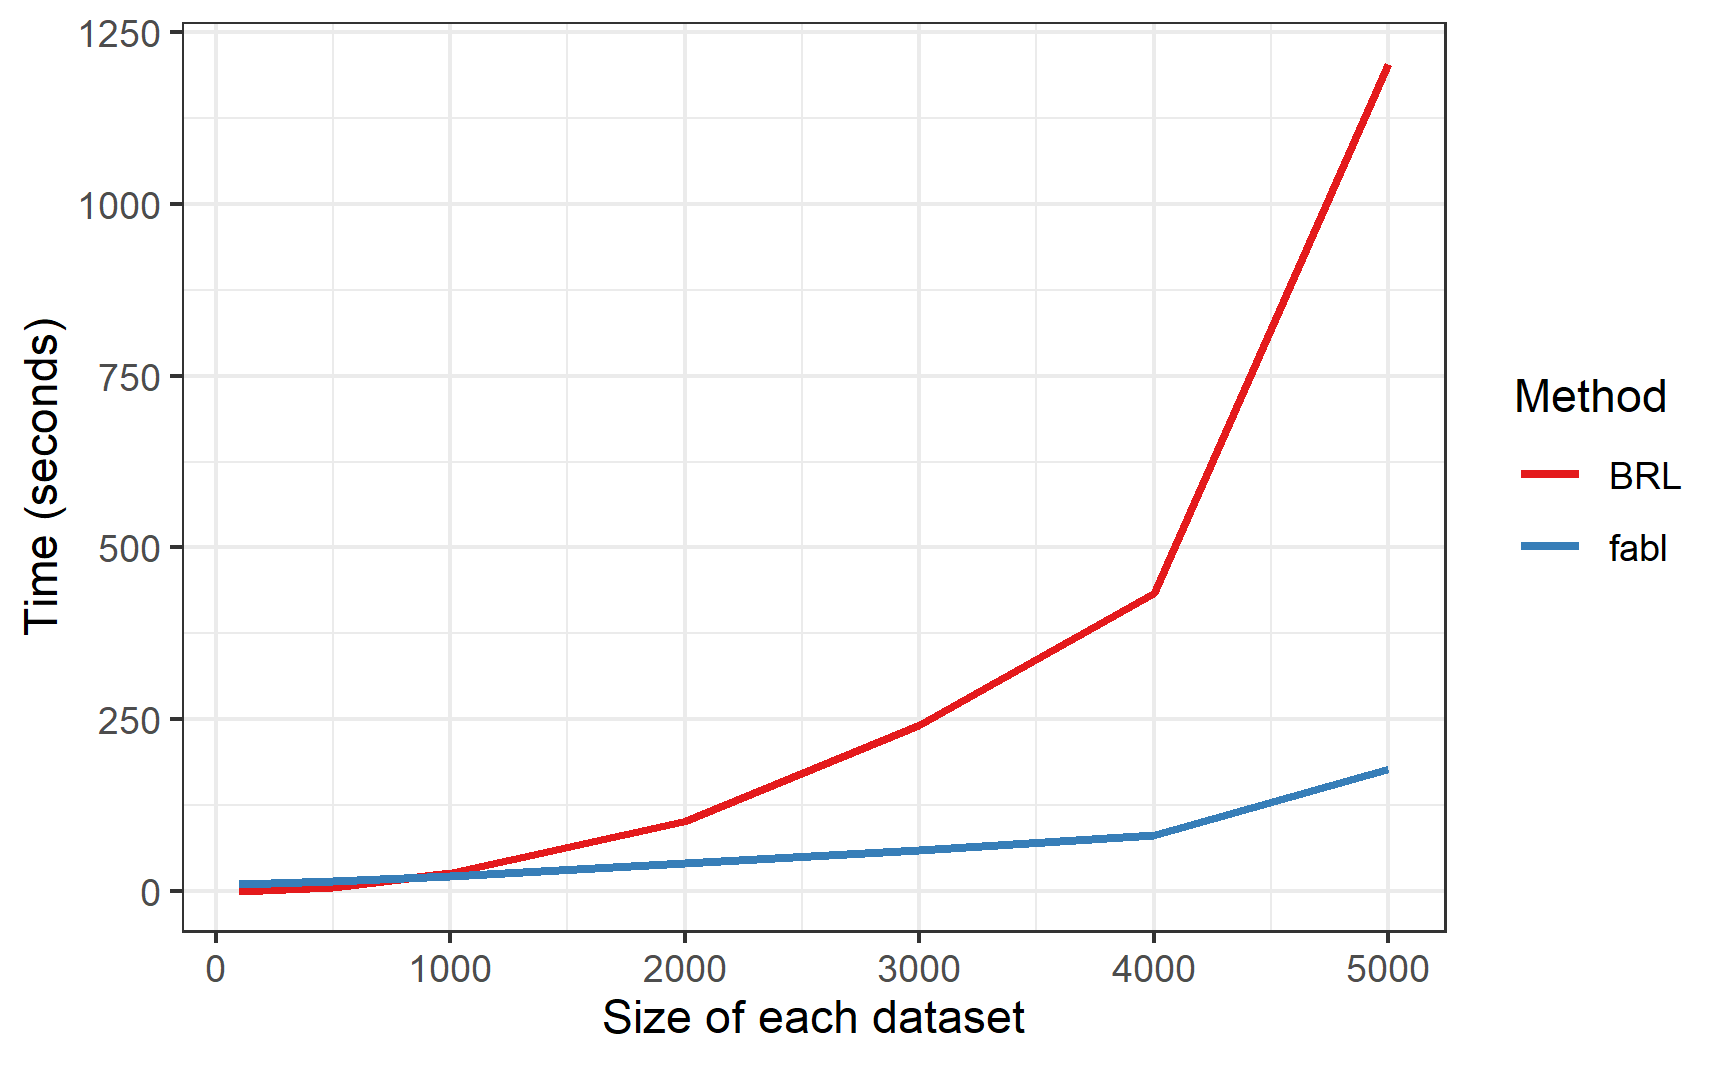
\includegraphics[width=0.7\textwidth]{finalFigures/figures/sadinle_speed_plot2}  
	 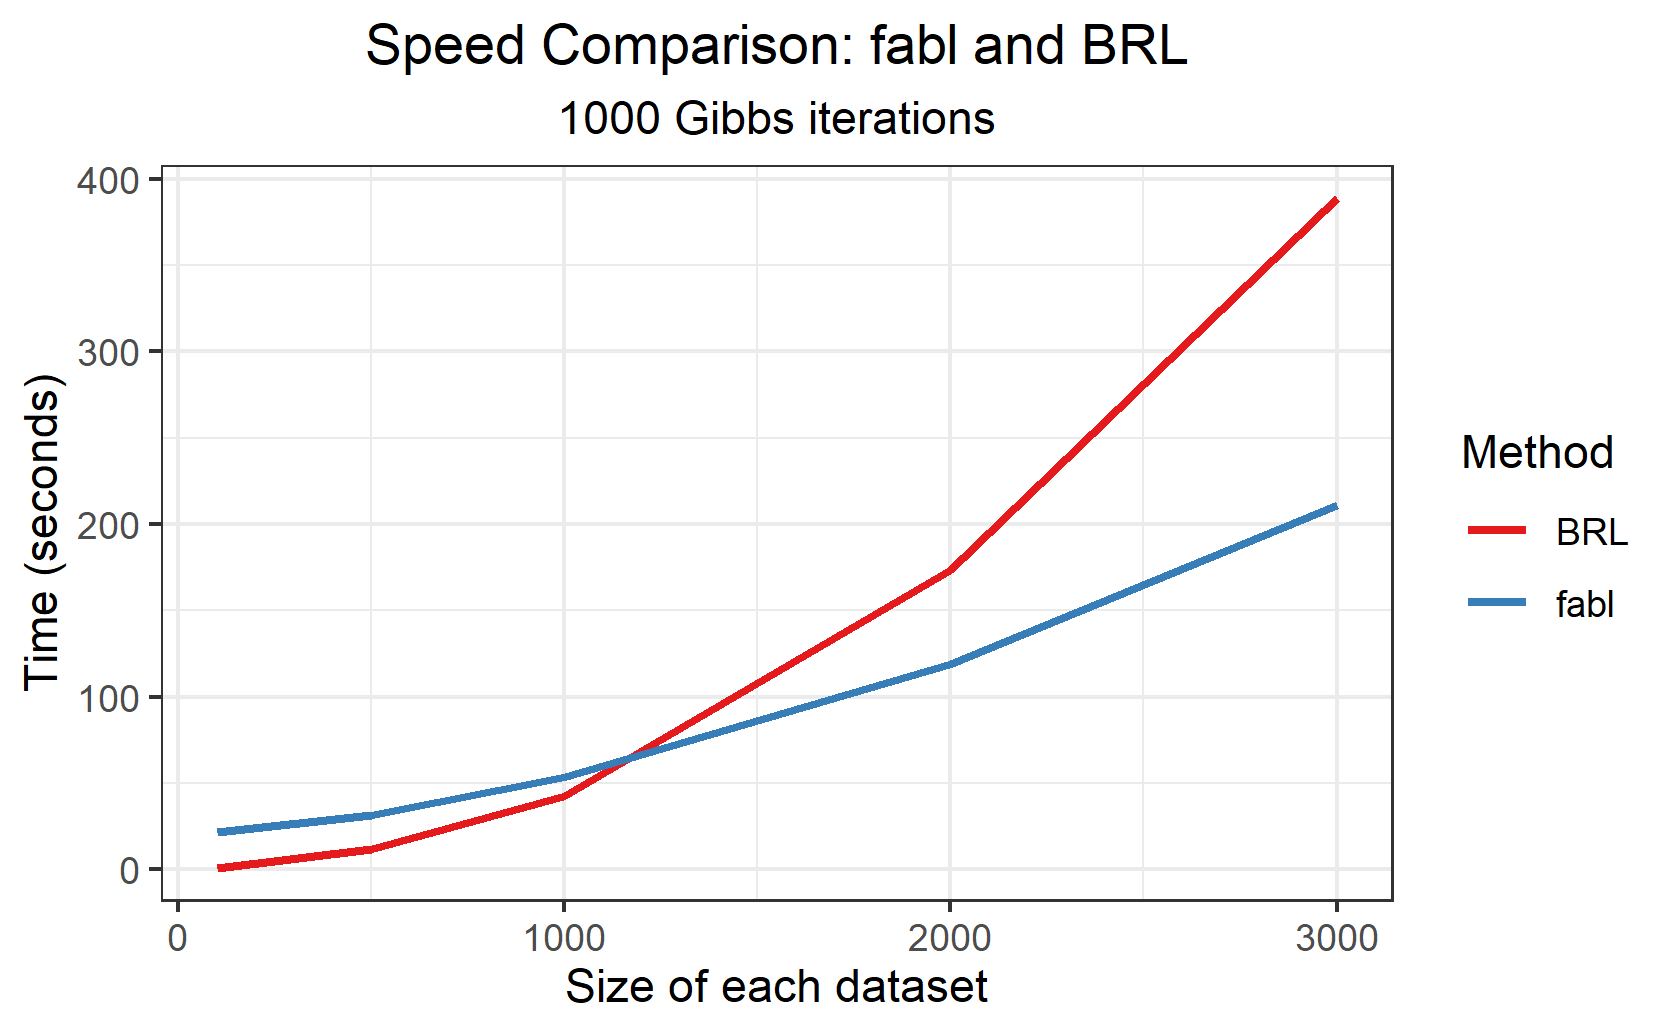
\includegraphics[width=0.7\textwidth]{../notes/figures/sadinle_speed_plot2} 
			\caption{Run-time for \texttt{BRL} and \texttt{fabl} to run 1000 Gibbs iterations, including the hashing step for \texttt{fabl}, for increasing values of both $n_A$ and $n_B$, as described in Section \ref{speed}. We see near quadratic growth in run-time for \texttt{BRL}, and near linear growth for \texttt{fabl}.}\label{fig:speed1}
		\end{center}
	\end{figure}
	
	In Figure \ref{fig:speed2}, where we fix $n_B = 500$, we see near linear growth for the run-time under \texttt{BRL} as $n_A$ increases, and much more static run-time under \texttt{fabl}. The slight increases in run-time for \texttt{fabl} are due primarily to the hashing step, which again can be run in parallel for large data. To illustrate that these trends are generalizeable to other specifications of the comparison vectors, we have included the run-time results for an additional simulation study, under different comparison vector settings, in Appendix \ref{app:appendix-speed}.
	
	Importantly, \texttt{BRL} implements a Gibbs sampler that is coded C \citep{sadinle_bayesian_2017}, while \texttt{fabl} currently uses non-optimized code written only in \texttt{R}.  While this complicates comparisons, and indeed disfavors \texttt{fabl}, the computational speed gains for \texttt{fabl} are still evident, especially for larger sample sizes.  Additionally, although \texttt{fabl} is amenable to parallelization, this simulation is run on a single core. Implementing \texttt{fabl} in C++ with parallelization for the hashing step and sampling the matching status of the record pairs should lead to even more computational gains.
	
	\begin{figure}[h!]
		\begin{center} 
%		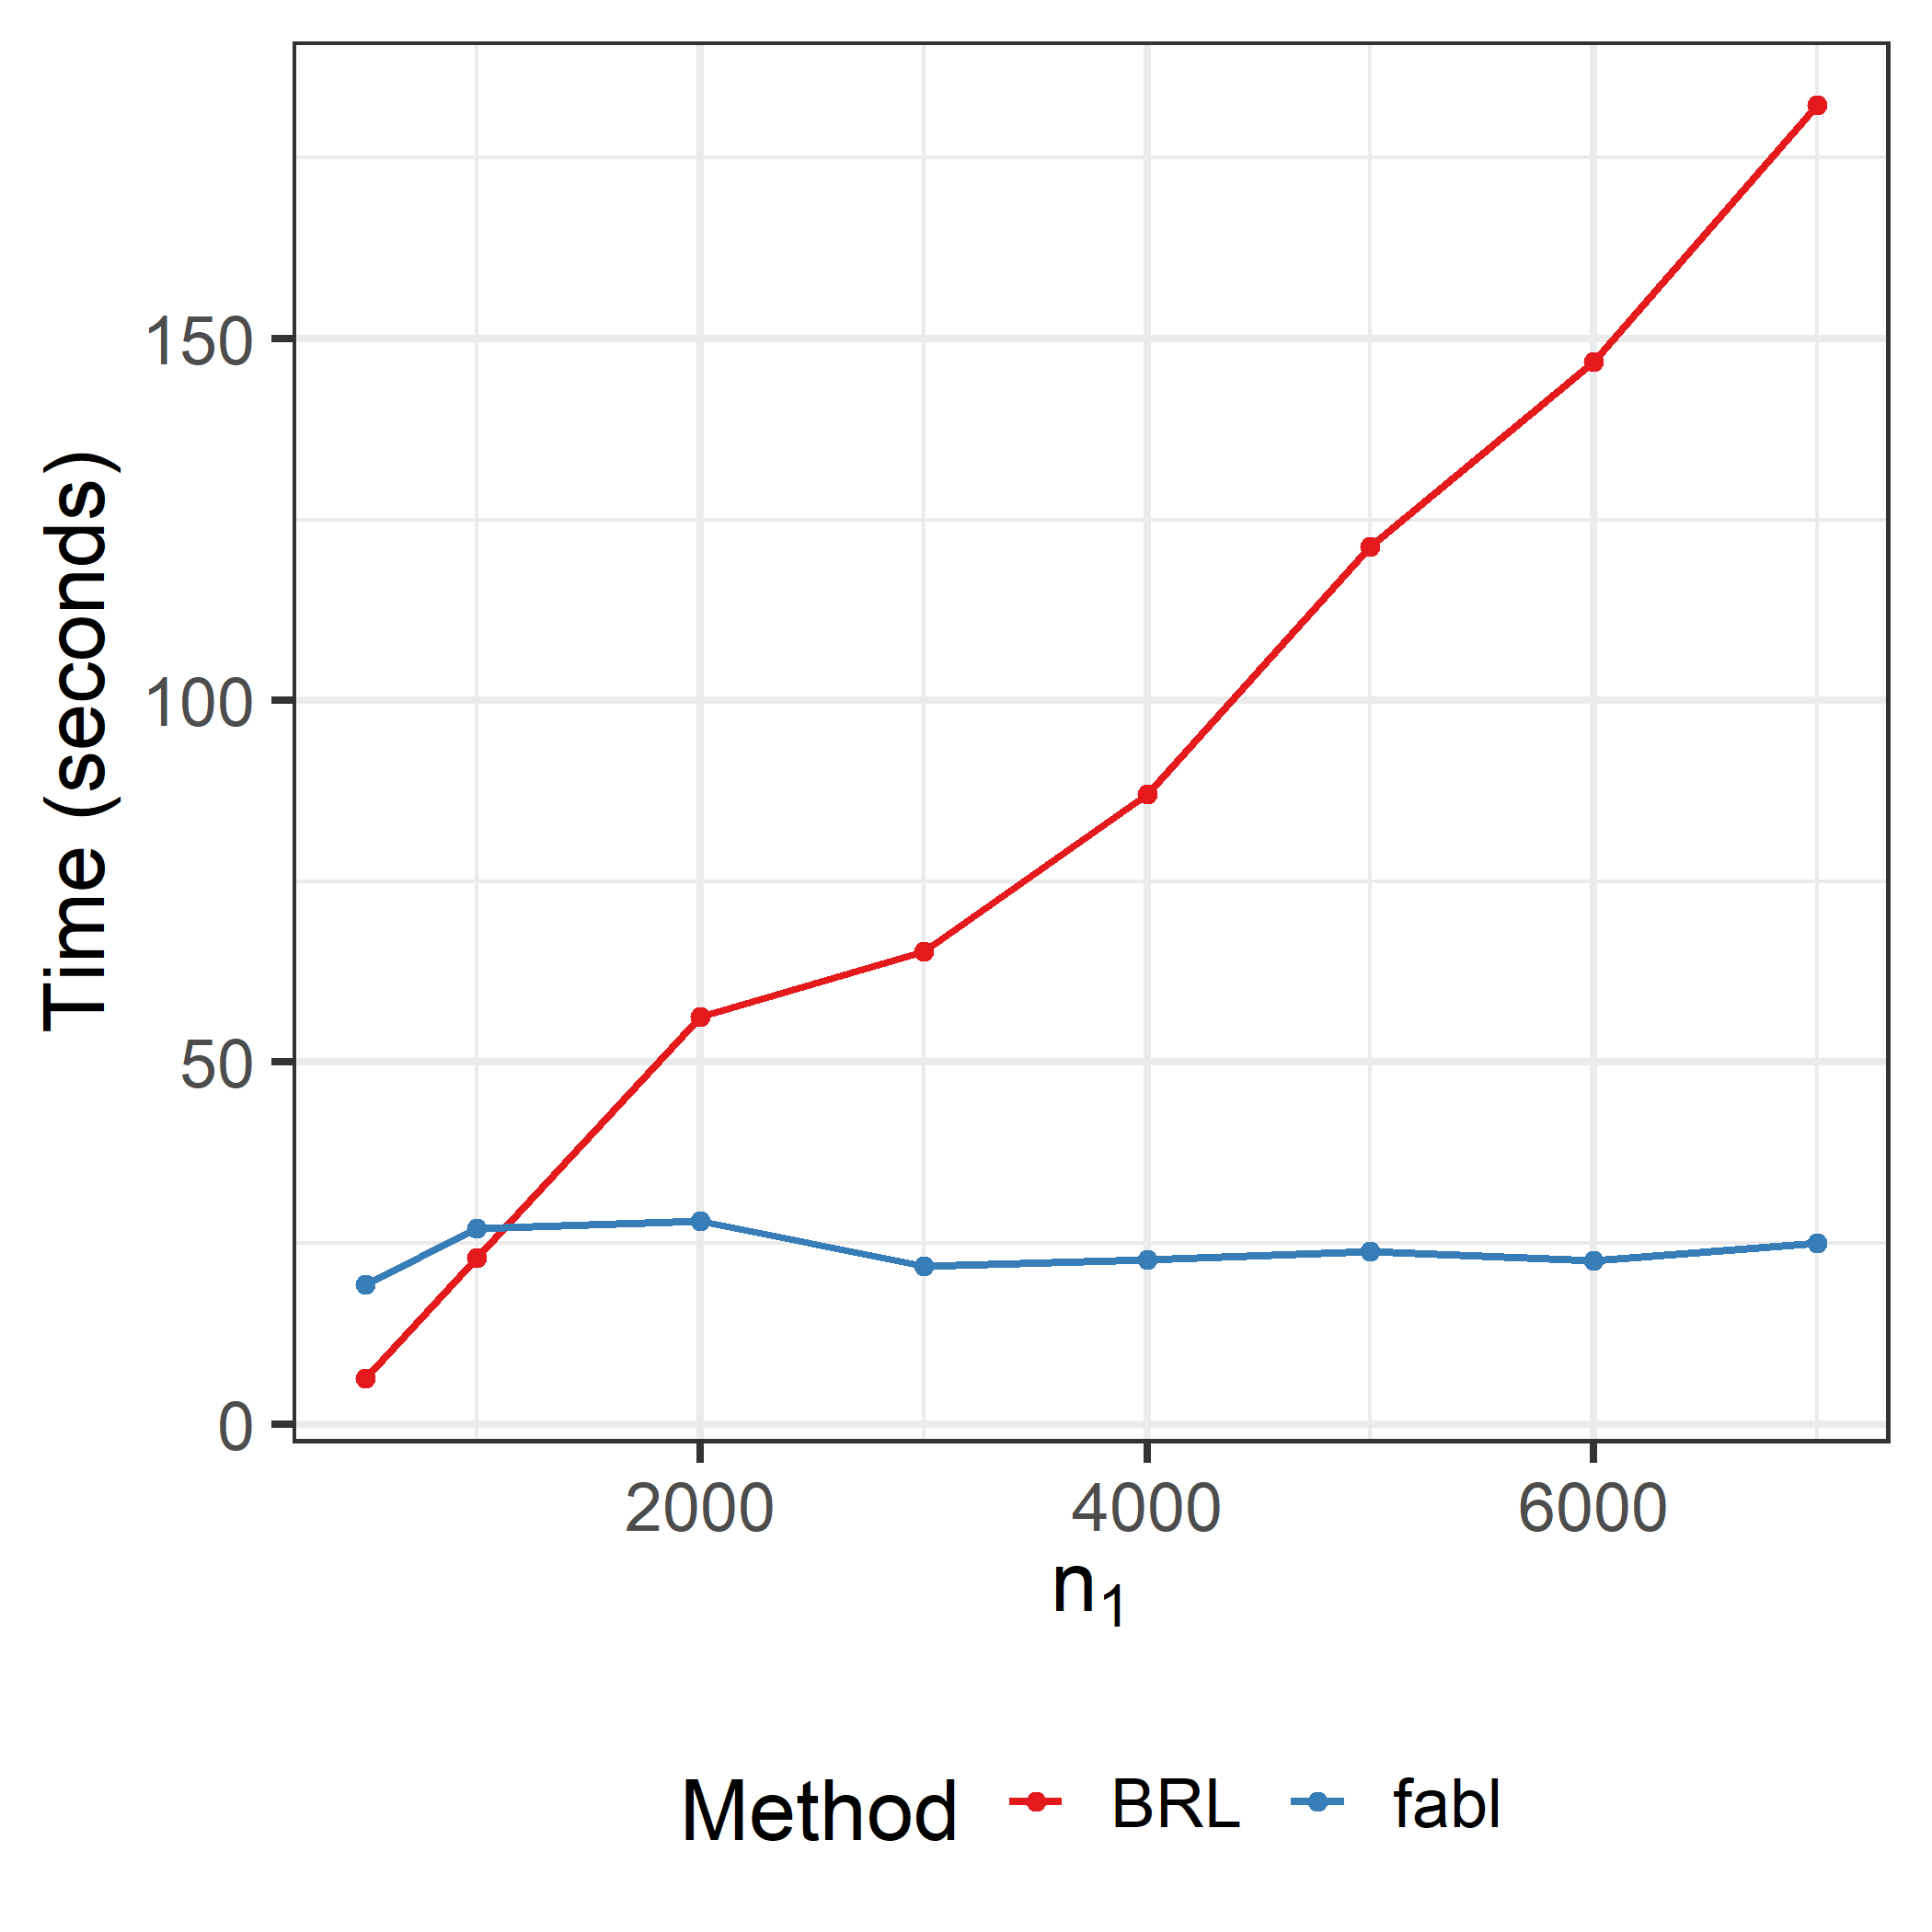
\includegraphics[width=0.7\textwidth]{finalFigures/figures/speed_plot_fixed_nB_slides} 
		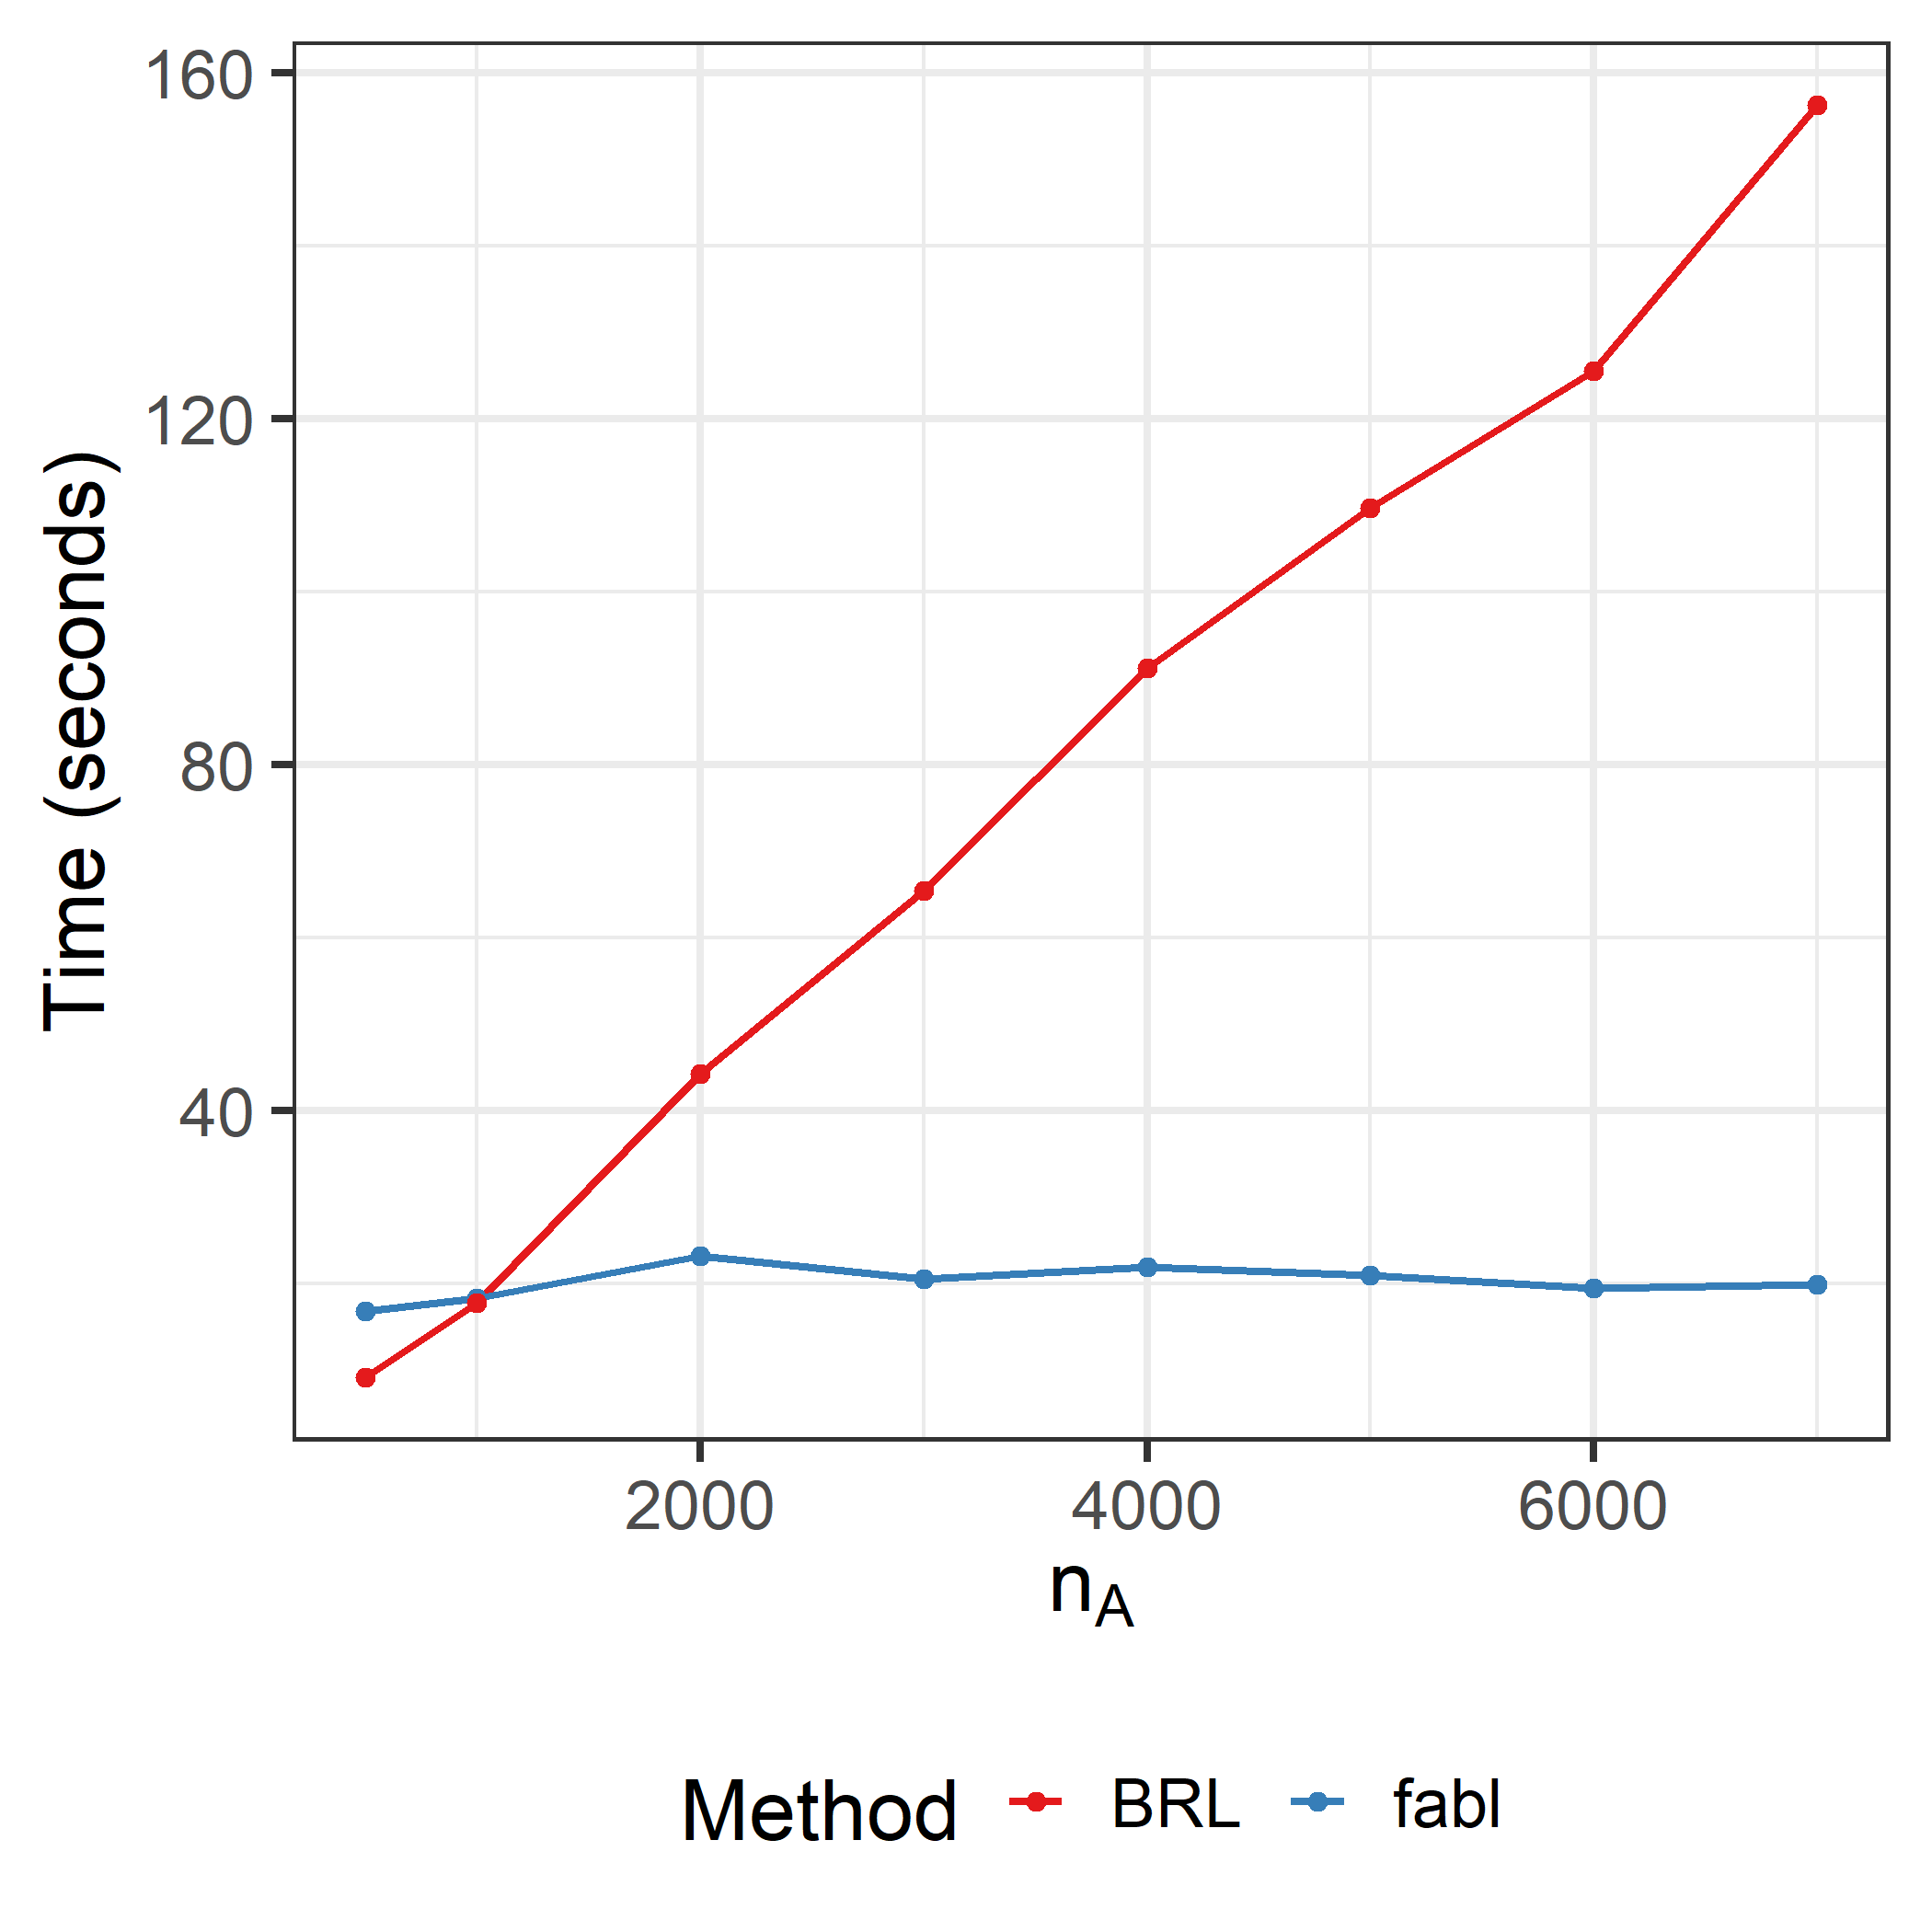
\includegraphics[width=0.7\textwidth]{../notes/figures/speed_plot_fixed_nB_slides} 
			\caption{Run-time for \texttt{BRL} and \texttt{fabl} to run 1000 Gibbs iterations, including hashing step for \texttt{fabl}, with $n_B$ fixed at 500, as described in Section \ref{speed}. We see near linear growth in run-time for \texttt{BRL}, and near constant run-time for \texttt{fabl}.}\label{fig:speed2}
		\end{center}
	\end{figure}
	
	
	\hypertarget{accuracy}{%
		\subsection{Accuracy}\label{accuracy}}
	
	Computational speed-ups are only worthwhile if not accompanied by a notable loss of record linkage accuracy. Therefore, we examine the accuracy of \texttt{fabl} relative to \texttt{BRL} by replicating a simulation study from \cite{sadinle_bayesian_2017}. The simulations employ a collection of synthetic data files with varying amounts of error and overlap (the number of records in common across files). Following methods proposed by \cite{christen_pudjijono2009} and \cite{christen_vatsalan2013}, clean records are first simulated from frequency tables for first name, last name, age, and occupation in Australia. Fields are then chosen for distortion uniformly at random. Names are subject to string insertions, deletions and substitutions, as well as common keyboard, phonetic, and optical recognition errors. Age and occupation are distorted through keyboard errors and missingness. These synthetic data files are available in the supplement to \cite{sadinle_bayesian_2017}.
	
	We create comparison vectors according to the default settings of the \texttt{compareRecords} function from the \texttt{BRL} package, shown in Table \ref{Tab:sadinle_simulation_cutoffs}. Each simulation identifies matched individuals between two data files, each with 500 records. We conduct linkage when matching records exhibit 1, 2, and 3 errors across the four fields, and when there are 50, 250, and 450 individuals in common across data files. Under each of these settings, we use 100 pairs of simulated data files in order to obtain uncertainty quantification on our performance metrics. We use uniform priors for all $\bm{m}$ and $\bm{u}$ parameters, with $\alpha_{fl} = \beta_{fl} = 1$ for all $f$ and $l$. We run the Gibbs sampler for 1000 iterations, and discard the first 100 as burn-in. We calculate Bayes estimates $\hat{\bm{Z}}$ of the linkage structure using the  loss function and post-processing procedure described in Appendix \ref{bayes-estimate}. Traceplots for parameters of interest for one example simulation are provided in Appendix \ref{app:appendix-sim}; they show no obvious concern over MCMC convergence. We also replicate this simulation allowing \texttt{fabl} to leave some components of the linkage structure undetermined and left for clerical review; those results are in Appendix \ref{partial}.
	
	\begin{table}[t]
		\centering
		\begin{tabular}[t]{llllll}
			
			\multicolumn{2}{c}{ } & \multicolumn{4}{c}{Level of Disagreement} \\
			\cline{3-6}
			Fields & Similarity & 1 & 2 & 3 & 4\\
			\hline
			First and Last Name & Levenstein & 0 & (0, .25] & (.25, .5] & (.5, .1]\\
			Age and Occupation & Binary & Agree & Disagree &  & \\
			\hline
		\end{tabular}
		\caption{Construction of comparison vectors for accuracy study with simulated data files of Section \ref{accuracy}.}
		\label{Tab:sadinle_simulation_cutoffs}
	\end{table}
	
	We compare \texttt{fabl} to \texttt{BRL} in terms of recall, precision and F-measure, as defined in \cite{christen_2012}. Recall is the proportion of true matches found by the model, that is, $\sum_{j=1}^{n_B} I(\hat{Z}_j = Z_j, Z_j \leq n_A) / \sum_{j=1}^{n_B} I(Z_j \leq n_A)$. Precision is the proportion of links found by the model that are true matches, that is, $\sum_{j=1}^{n_B} I(\hat{Z}_j = Z_j, Z_j \leq n_A) / \sum_{j=1}^{n_B} I(\hat{Z}_j \leq n_A)$. The F-measure balances the two metrics to provide an overall measure of accuracy, and is defined as $2  (\text{Recall } + \text{ Precision}) / (\text{Recall } \times \text{ Precision})$. In Figure \ref{fig:sadinle_simulation}, we see that the two methods have comparable performance at all levels of error and overlap. In the specific case of high error and low overlap, widely regarded as the most difficult linkage scenario, we see that \texttt{fabl} performs slightly worse than \texttt{BRL} on average; however, the overall accuracy level remains high. 
	
	\begin{figure}[t]
		\begin{center}
%		\includegraphics[width=0.7\textwidth]{finalFigures/figures/sadinle_sim_plot2} 
			\includegraphics[width=0.7\textwidth]{../notes/figures/sadinle_sim_plot2} 
			\caption{Posterior means and credible intervals for accuracy metrics under the replication of simulation study from \cite{sadinle_bayesian_2017}. For each level of overlap and each level of error, we have 100 paired sets of 500 records. Thus this table summarizes results for 900 data files. We see comparable performance for all levels of error and overlap.}
			\label{fig:sadinle_simulation}
		\end{center}
	\end{figure}

	\hypertarget{SEI-sensitivity}{%
	\subsection{SEI Sensitivity}\label{SEI-sensitivity}}

Finally, our last simulation demonstrates our method's robustness to different values of $S$ for the SEI memory reduction procedure. We perform record linkage on one set of synthetic datafile described in Section \ref{accuracy} with 500 records in each datafile, 250 entities in common across datafiles, and 3 errors present across matching records. To achieve more drastic results, we perform SEI without chunking the data, that is, $t_A = t_B = 1$. In practice, if it is possible to create and store the comparison matrix for all record pairs at one time, there is no need to reduce the memory of the hashed matrix through SEI. For illustration however, it is easier to illustrate the effects of choices of $S$ in this setting. 

We preform linkage using SEI with $S = (1, 2, 5, 10, 20)$, and without using SEI, always with 500 iterations of the Gibbs sampler. As any particular SEI implementation may improve or worsen linkage performance; if the SEI procedure happens to only remove pairs that are not matches, recall and precision will improve. Therefore, we perform linkage under each setting 100 times, recording the linkage estimate $\hat{\bm{Z}}$, and recall and precision.

In Figure \ref{fig:SEI_Z}, the largest number of distinct linkage estimates occurs when $S = 1$. This makes sense, because the SEI procedure arbitrarily removes large numbers of record labels from consideration, resulting in a noisier estimate of the linkage structure. The number of distinct linkage estimates decreases as $S$ increases, with larger values of $S$ providing results more similar to the linkage without SEI. In Figure \ref{fig:SEI_eval}, we see similar patterns in precision. Setting $S=1$ can arbitrarily remove the index of a true match, leading the Gibbs sampler to concentrate probability on a false match, while larger values of $S$ produce results mirroring implementation with no SEI. We note however that even with $S=1$, the loss in precision is small.

Although the figures suggest that $S=2$ is adequate for maintaining linkage performance, we suggest a more conservative value like $S=10$. When evaluating the performance of a record linkage algorithm, researchers often examine posterior probabilities. By concentrating probability mass on arbitrary nonmatches, low values of $S$ may induce suspiciously high posterior probability for certain record pairs, providing a misleading perception of model performance. 


\begin{figure}
	\begin{minipage}[c]{0.4\linewidth}
		\begin{center}
%		\includegraphics[width=\linewidth]{finalFigures/SEI_sensitivity/Z_plot}
		\includegraphics[width=\linewidth]{../SEI_sensitivity/Z_plot}
		\caption{Distinct values of $\hat{Z}$ in Section \ref{SEI-sensitivity} simulation.}
		\label{fig:SEI_Z}
		\end{center}
	\end{minipage}
	\hfill
	\begin{minipage}[c]{0.5\linewidth}
		\begin{center}
		\includegraphics[width=\linewidth]{finalFigures/SEI_sensitivity/eval_plot} 
%	\includegraphics[width=\linewidth]{../SEI_sensitivity/eval_plot} 
		\caption{Means and 95\% credible intervals for recall and precision in Section \ref{SEI-sensitivity} simulation.}
		\label{fig:SEI_eval}
	\end{center}
	\end{minipage}%
\end{figure}
	\section{Case Studies}
	\label{sec:case-studies}
	
	In our first case study, we revisit data from the El Salvadoran Civil War analyzed by \cite{sadinle_bayesian_2017} and others \citep{lum2013applications, jewell2018accounting}. Though the data files used in this case study are small, it shows how the computational complexity of \texttt{fabl} depends on the number of unique agreement patterns found in the data, and how significant computational gains can be achieved by simplifying the construction of the comparison vectors. In the second case study, we apply \texttt{fabl} to link records from the National Long Term Care Study, a larger linkage task that is not feasible in reasonable time under \texttt{BRL} with typical computing setups. 
	
	\subsection{Civilian Casualties from the El Salvadoran Civil War}
	\label{el_salvador}
	
	The country of El Salvador was immersed in civil war from 1980 to 1991. We are interested in estimating the total number of casualties from the war. We utilize lists of casualties from the war, one collected by El Rescate - Tutela Regal (ERTL)\citep{howland2008rescate} and another from the Salvadoran Human Rights Commission (CDHES, by its acronym in Spanish)\citep{ball2000salvadoran}.\footnote{We thank the Human Rights Data Analysis Group (HRDAG) for granting access to these data.} The ERTL dataset comprises digitized denunciations published throughout the conflict, and the CDHES dataset comprises casualties reported directly to the organization. The ERTL required additional investigation before recording denunciations as human rights abuses, and reports to the CHDES were made shortly after the events occurred; thus, both data files are thought to be fairly reliable. When estimating the total number of casualties, one cannot simply sum the numbers recorded by each organization, as it is likely that the same individuals are recorded in multiple casualty lists. Instead, record linkage techniques must be used to merge data files before analyzing the data \citep{lum2013applications}. 
	
	There are several challenges with these data. First, both data files have been automatically digitized, which inherently leads to some degree of typographical error. Second, the only fields recorded are given name, last name, date of death, and place of death. \textcolor{teal}{While it may be common in other data sets for a parent and child to share the same given name, in this data set, it is more common for cousins to share this information, especially in villages, where there may be only four to five extended families. In Latin America, an individual receives a surname from their father and their mother, leading to a limited number of surnames in small villages.}
	%% I believe that Patrick said that this is not common in this data set
%	It is relatively common for a parent and child to share the same given name, resulting in indistinguishable records for two different individuals. 
	
	Following \cite{sadinle_bayesian_2017}, we utilize records that have non-missing entries for given and last name, which results in $n_A = 4420$ records in CHDES and $n_B = 1323$ records in ERTL. We standardize names to account for common misspellings and use a modified Levenstein distance when comparing names to account for the fact that second names are often omitted in Spanish. Place of death is recorded by municipality and department within that municipality; however, since department is missing in 95\% of records in CHDES and 80\% of records in ERTL, we exclude department from our analysis. Thus, we conduct record linkage using given name, last name, municipality, and day, month, and year of death. We use uniform priors for the $\bm{m}$ and $\bm{u}$ parameters.
	
	We initially followed the comparison vector constructions set by \cite{sadinle_bayesian_2017}, using four levels of agreement for each field, according to the thresholds provided in Table \ref{Tab:el_salvador_cutoffs_1}. This results in $5^5 \times 3 = 6025$ possible agreement patterns, with 1173 patterns realized in the data. However, we noticed that the posterior distributions of several levels of the $\bm{m}$ and $\bm{u}$ parameters were nearly identical in an initial run of \texttt{BRL}, suggesting that these levels were unnecessary.
	
	\begin{table}[t]
		\begin{tabular}[t]{llllll}
			\multicolumn{2}{c}{ } & \multicolumn{4}{c}{Level of Disagreement} \\
			\cline{3-6}
			Fields & Similarity & 1 & 2 & 3 & 4\\
			\hline
			First and Last Name & Modified Levenstein & 0 & (0, .25] & (.25, .5] & (.5, 1]\\
			Year of Death & Absolute Difference & 0 & 1 & 2 & 3+\\
			Month of Death & Absolute Difference & 0 & 1 & 2-3 & 4+\\
			Day of Death & Absolute Difference & 0 & 1-2 & 3-7 & 8+\\
			Municipality & Binary & Agree & Disagree &  & \\
			\hline
		\end{tabular}
		\caption{Construction of comparison vectors for El Salvador data resembling original implementation from \cite{sadinle_bayesian_2017}. This setup leads to 2048 possible agreement patterns in total.}\label{Tab:el_salvador_cutoffs_1}
	\end{table}

	\begin{table}[t]
	\centering
	\begin{tabular}[t]{lllll}
		\multicolumn{2}{c}{ } & \multicolumn{3}{c}{Level of Disagreement} \\
		\cline{3-5}
		Fields & Similarity & 1 & 2 & 3\\
		\hline
		First and Last Name & Modified Levenstein & 0 & (0, .25] & (.25, 1]\\
		Year of Death & Binary & Agree & Disagree & \\
		Month of Death & Binary & Agree & Disagree & \\
		Day of Death & Absolute Difference & 0 & 1 & 2+\\
		Municipality & Binary & Agree & Disagree & \\
		\hline
	\end{tabular}
	\caption{Construction of comparison vectors for El Salvador data for increased speed under \texttt{fabl}. This setup leads to 216 possible agreement patterns in total.}\label{Tab:el_salvador_cutoffs_2}
\end{table}
	
	Therefore, we perform our analysis with the agreement levels for each field according to Table \ref{Tab:el_salvador_cutoffs_2}. Among the 216 possible agreement patterns, 159 are realized in the data. With this revised comparison specification, \texttt{fabl} runs in 61 seconds, approximately 4 times faster than the \texttt{BRL} run time of 239 seconds.  The estimates of the $\bm{m}$ parameters under each method are similar, as shown in Figure \ref{fig:m-and-u}. Estimates of $\bm{u}$ are indistinguishable, and thus omitted. Traceplots for parameters of interest are provided in Appendix \ref{app:appendix-es}.
	
	For completeness, we note that linkage with the more detailed comparison vectors requires 240 seconds for \texttt{BRL}, and 261 seconds for \texttt{fabl}.  Apparently, the number of patterns is sufficiently many that the computational savings from \texttt{fabl} does not overcome the inherent speed differences of C as opposed to \texttt{R}.
	
	Through \texttt{fabl}, we arrive at a Bayes estimate of 179 individuals recorded in both data files. We calculate posterior samples of the size of the overlap across files by finding the number of links in each iteration of the Gibbs sampler, and subtracting the number of matches that violate one-to-one matching. The posterior 95\% credible interval for the overlap across files is (206, 238), indicating that the Bayes estimate identifies fewer matches than the Gibbs sampler identifies on average. This is because a large number of records in ERTL have multiple plausible matches in CDHES; \texttt{fabl} recognizes that a match exists among the several options, but is unable to definitely declare a specific pair as a match in the Bayes estimate. We see similar results under \texttt{BRL}, with a Bayes estimate of 181 individuals recorded in both data files, and a posterior 95\% credible interval of (211, 244). See Figure \ref{fig:overlap-plot} for a visual comparison of the Bayes estimates and posterior credible intervals for the two methods. We note that Bayes estimates falling outside of posterior credible intervals has been observed previously in the record linkage literature \citep{sadinle_bayesian_2017, steorts_bayesian_2016}, and remains a topic for future research.
	

	
	\begin{figure}[t]
		\begin{center}
%		         \includegraphics[width=0.6\textwidth]{finalFigures/el_salvador/overlap_distribution_smallP_bayes}
	\includegraphics[width=0.6\textwidth]{../notes/figures/el_salvador/overlap_distribution_smallP_bayes}
			\caption{Posterior distribution and Bayes estimate of overlap across the two files. We note they are quite similar under both methods.}
			\label{fig:overlap-plot}
		\end{center}
	\end{figure}
	
	
	\begin{figure}[t]
		\begin{center}
%		         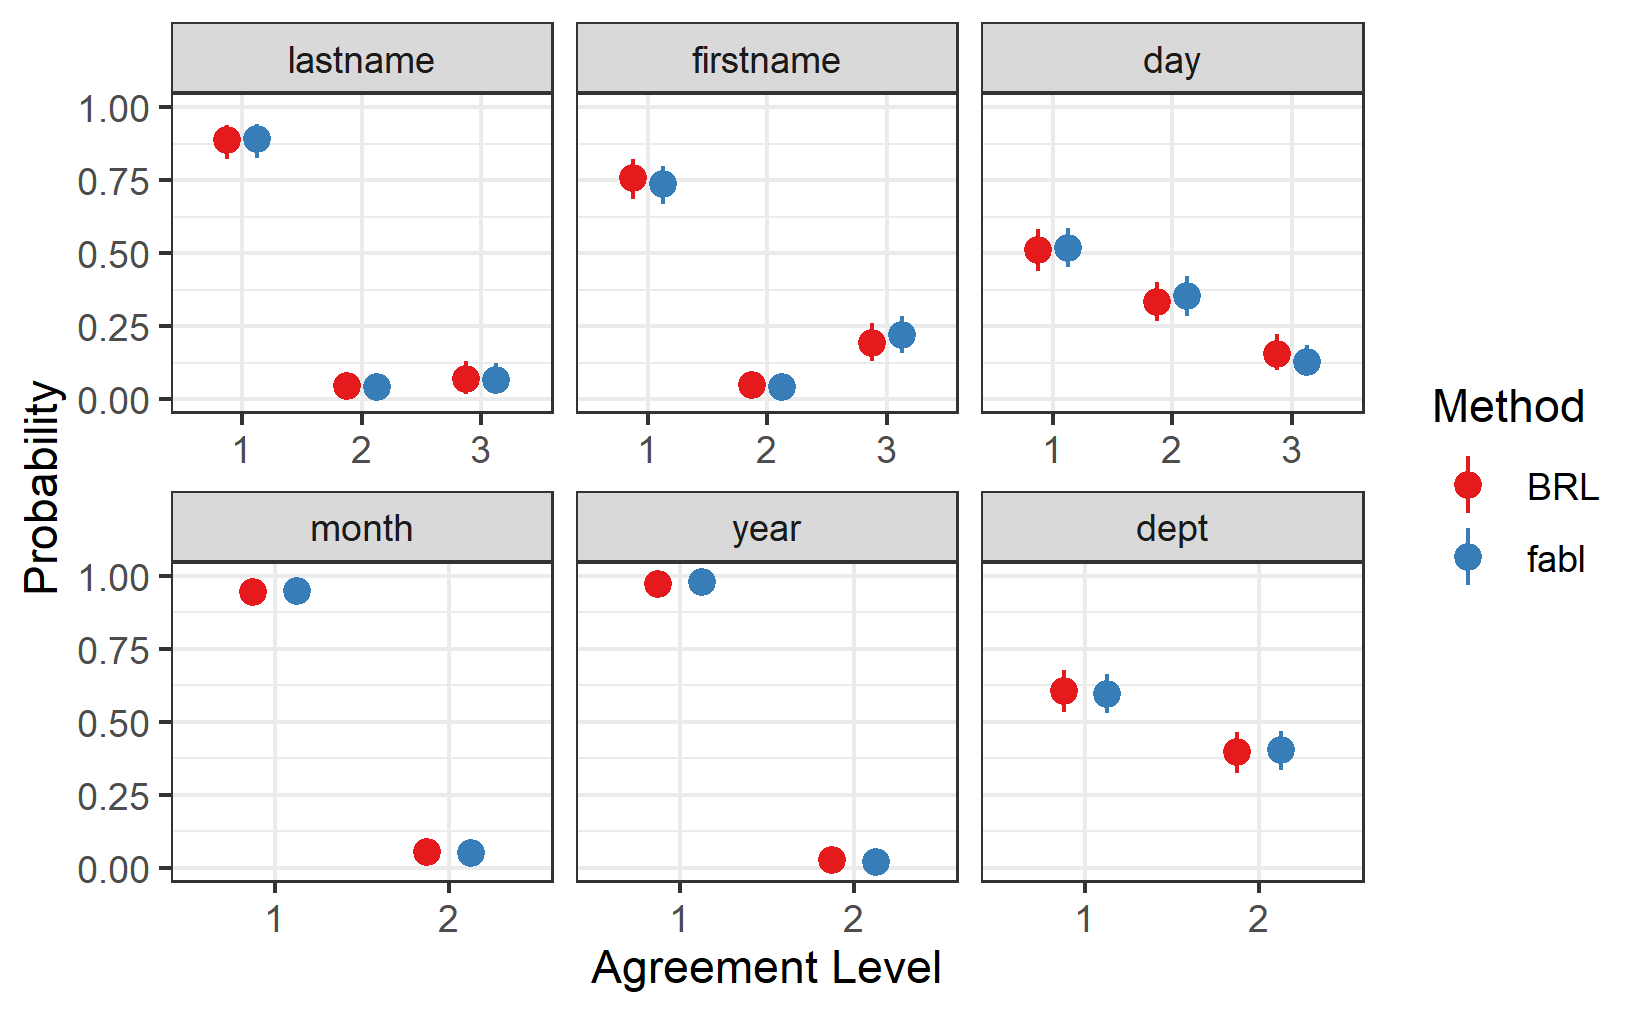
\includegraphics[width=0.6\textwidth]{finalFigures/el_salvador/m_posterior_smallP} 
                  	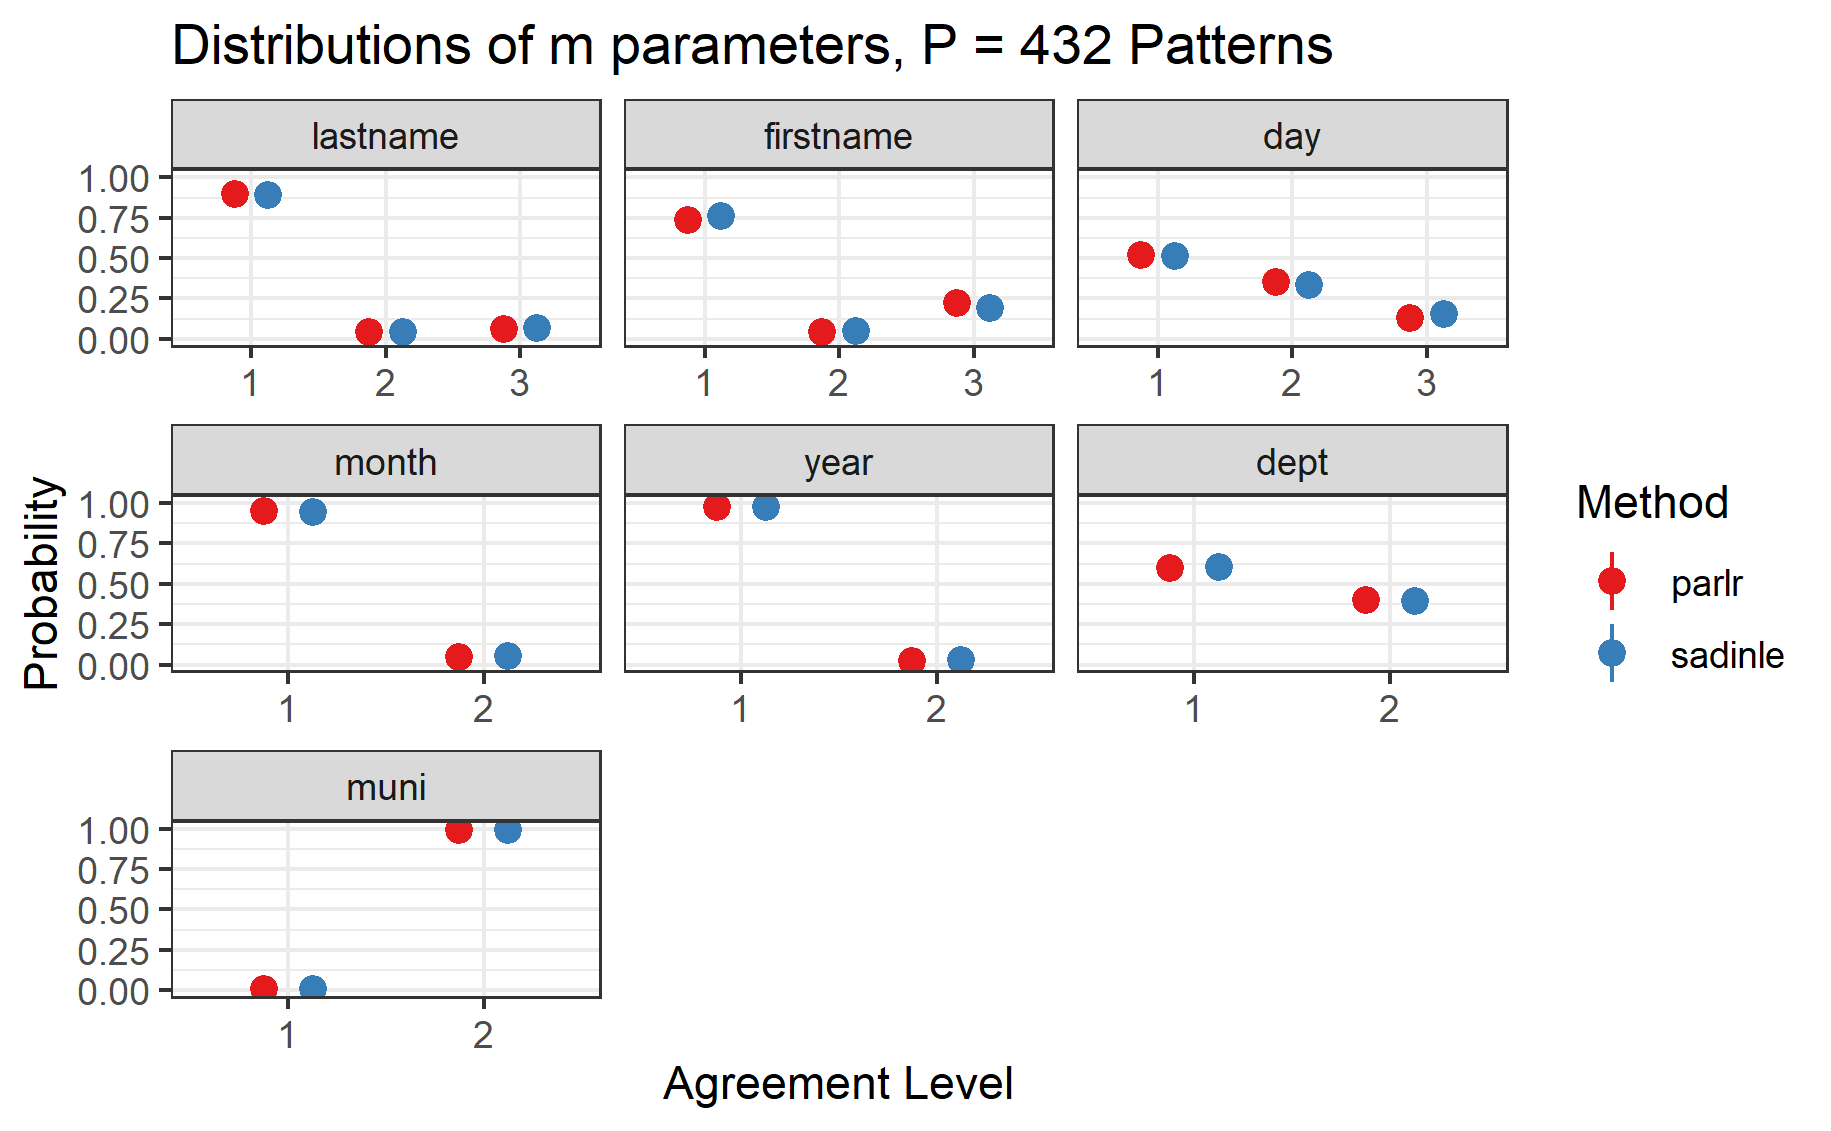
\includegraphics[width=0.6\textwidth]{../notes/figures/el_salvador/m_posterior_smallP} 
			\caption{Posterior estimates of $\bm{m}$ parameters with 95\% credible intervals for the El Salvador case study. They are quite similar across the two methods.}\label{fig:m-and-u}
			\label{fig:m-and-u}
		\end{center}
	\end{figure}
	
	\subsection{National Long Term Care Study}
	\label{nltcs}
	
	\begin{table}[t]
		\centering
		\begin{tabular}[t]{lllll}
			\multicolumn{2}{c}{ } & \multicolumn{3}{c}{Level of Disagreement} \\
			\cline{3-5}
			Fields & Similarity & 1 & 2 & 3\\
			\hline
			Sex & Binary & Agree & Disagree & \\
			Year of Birth & Binary & Agree & Disagree & \\
			Month of Birth & Binary & Agree & Disagree & \\
			Day of Birth & Binary & Agree & Disagree & \\
			Location & Custom & Same State and Office & Same State & Otherwise \\
			\hline
		\end{tabular}
		\caption{Construction of comparison vectors for NTLCS data.}\label{Tab:nltcs-comparisons}
	\end{table}
	
	The National Long Term Care Study (NLTCS) is a longitudinal study tracking the health outcomes of Medicare recipients \citep{steorts_bayesian_2016}. The initial survey began in 1982, with follow-up surveys taken approximately every five years. As such, patients are surveyed at most once in a given year, and many patients are surveyed across multiple years. In addition, patients can either drop out of the study, pass away, or enter as new patients. Hence, the assumptions of our model hold for this study. We seek to link records over the $n_A = 20485$ individuals from 1982 to the $n_B = 17466$ individuals from 1989. The NLTCS data have longitudinal links, so that in reality one does not need to conduct record linkage. However, following the strategy in \cite{guha:reiter:BA}, we break the longitudinal links and treat the data from 1982 and 1989 as stand-alone data files.
	
	We link records using sex, date of birth, and location using the thresholds shown in Table \ref{Tab:nltcs-comparisons}. Storing $\gamma$ constructed through three comparison scores for each of $20485 (17466) \approx 400,000,000$ record pairs would require approximately 8GB of memory. Standard settings on a 16GB personal computer do not allow storage of an object of this size, and thus \texttt{BRL} is unable to perform this linkage task on such a machine. {\color{red}{However, through the method described in Section \ref{scaling},  we perform 30 smaller comparison tasks, using $t_A = 1$ and $t_B = 30$. We conduct linkage with all record indices recorded and also with SEI using $S=10$, and obtain identical results. The hashed $\tilde{\gamma}$ without SEI is about 2.2 GB, and with SEI, it is about 760 MB. Constructing the comparisons sequentially took approximately 40 minutes, which could be reduced considerably through parallel computing.}}
	
	We run a Gibbs sampler for 1000 iterations, taking about 235 seconds. As shown in Figure \ref{fig:nltcs-overlap-plot}, the Bayes estimate of the linkage structure consists of 9634 matches, with a 95\% credible interval of (9581, 9740). Since we have access to the true linkage structure, we can calculate recall to be 0.89 and precision to be 0.98, resulting in an F-measure of 0.94. Traceplots do not suggest convergence issues, and are similar to those seen in Appendix \ref{app:appendix-sim} and \ref{app:appendix-es}
	
	\begin{figure}[h]
		\begin{center}
%		        \includegraphics[width=0.6\textwidth]{finalFigures/nltcs/overlap_posterior4}
 		\includegraphics[width=0.6\textwidth]{../notes/figures/nltcs/overlap_posterior4}
			\caption{Posterior distribution and Bayes estimate of overlap across years 1982 and 1989 of NLTCS data.}
			\label{fig:nltcs-overlap-plot}
		\end{center}
	\end{figure}
	
	
	\section{Conclusion}
	\label{discussion}
	
	In this paper, we have proposed \texttt{fabl}, a Bayesian record linkage method that extends the work of \cite{sadinle_bayesian_2017} to scale to large data sets. We have proven that the proposed hashing method and model assumptions allow for a linkage procedure whose computational complexity does not scale with the size of the larger data file. This makes \texttt{fabl} computationally advantageous in many linkage scenarios, particularly when one data file is substantially smaller than the other. We have also shown that storage efficient indexing, in tandem with hashing, greatly reduces the memory costs required for all-to-all comparisons, giving practitioners an option for larger record linkage tasks potentially even without the use of blocking or indexing. We have demonstrated the speed and accuracy of \texttt{fabl} by replicating a simulation study and a case study in \cite{sadinle_bayesian_2017}, and through an additional case study that is computationally impractical under \texttt{BRL}. 
	
	Although the \texttt{fabl} method greatly reduces the memory costs for all-to-all comparisons, computing all $n_A  n_B$ record pairs still can be prohibitive for larger linkage tasks. Indeed, constructing the comparison vectors for the NLTCS linkage task involving around 40,000 records in Section \ref{nltcs} took around 40 minutes. Due to the quadratic nature of the comparison space, this computation time would grow quickly with the size of the linkage task, and would be infeasibly slow when dealing with millions of records. Although it is common to use deterministic blocking to reduce the comparison space and then apply probabilistic record linkage within each block, issues arise when sizes of blocks vary across the linkage task. In future work, we seek to extend \texttt{fabl} to account for such deterministic blocking, making the framework amenable to even larger linkage tasks.
	
\begin{supplement}
\stitle{Supplementary Material of ``Efficient and Scalable Bipartite Matching with
Fast Beta Linkage (fabl)." See the .pdf document}
\sdescription{}
\end{supplement}



	
	\clearpage
	
	\bigskip
	
	\bibliographystyle{jasa}
	\bibliography{fabl}
	

	

%\appendix
%	
%		
%	
%	\hypertarget{app:derivations}{%
%	\section{Derivations of Full Conditionals}\label{app:derivations}}
%\textcolor{red}{Note: Please use s, s+1 consistently throughout. Or surpress the notation and tell the reader. It looks weird to go back and forth. I've tried to provide an intermediate solution. Perhaps Jerry can state if he would think this is okay as an Editor.}\\
%
%\textcolor{teal}{We provide detailed derivations of the full-conditionals provided in Section~\ref{sec:fast-beta-linkage}. In our derivations below, we assume that the new update to the Gibbs sampler is $s+1$ and the current state of the sampler is $s.$ As to not overload notation, we suppress the state of the sampler until presenting the final update of the full conditional that appears in Section~\ref{sec:fast-beta-linkage}.}
%
%The $\bm{m}$ and $\bm{u}$ parameters are updated through standard multinomial-Dirichlet distributions. For a particular $m_{fl}$, we have
%\begin{align*}
%	\mathcal{L}(m_{fl}|\gamma, \alpha_{fl}, \bm{u}, \bm{Z}, \pi) &\propto \prod_{i=1}^{n_A} \prod_{j=1}^{n_B} m_{fl}^{I(Z_j = i) I(\gamma_{ij}^f = l) I_{obs}(\gamma_{ij}^f)}  m_{fl}^{\alpha_{fl} - 1} = m_{fl}^{\alpha_{fl}(\bm{Z}) - 1},
%\end{align*}
%where $\alpha_{fl}(\bm{Z})= \alpha_{fl} + \sum_{i,j} I_{obs}(\gamma_{ij}^f)I(\gamma_{ij}^f = l) I(Z_j = i)$. Analogous procedures lead to the posterior distribution $\mathcal{L}(u_{fl}| \gamma, \beta_{fl}, \bm{m}, \bm{Z}, \pi)$  $\propto u_{fl}^{\beta_{fl}(\bm{Z}) - 1}$, where $\beta_{fl}(\bm{Z})= \beta_{fl} + \sum_{i,j} I_{obs}(\gamma_{ij}^f)I(\gamma_{ij}^f = l) I(Z_j \neq i)$. Thus for the vectors of parameters $\bm{m}_f$ and $\bm{u}_f$, we have
%
%$$\bm{m}_f^{(s+1)}|\bm{Z}^{(s)}, \gamma \sim \text{Dirichlet}(\alpha_{f1}(\bm{Z}^{(s)}), \ldots, \alpha_{fL_f}(\bm{Z}^{(s)})),$$
%$$\bm{u}_f^{(s+1)}|\bm{Z}^{(s)}, \gamma \sim \text{Dirichlet}(\beta_{f1}(\bm{Z}^{(s)}), \ldots, \beta_{fL_f}(\bm{Z}^{(s)})).$$
%
%Since $\pi$ encodes the rate of matching across the two data files, the full conditional $p(\pi|\gamma, \bm{Z}, \bm{m}, \bm{u}, \alpha_{\pi}, \beta_{\pi})$ depends only on the number of links $n_{AB}(\bm{Z}) = \sum_{i=1}^{n_B}I(Z_j < n_A + j)$ encoded by $\bm{Z}$ and hyperparameters. We have the full conditional
%\begin{align*}
%	p(\pi | \bm{Z}, \alpha_{\pi}, \beta_{\pi}) &\propto p(\bm{Z}|\pi)p(\pi) \\
%	&\propto \pi^{n_{AB}(\bm{Z})} (1-\pi)^{n_B - n_{AB}(\bm{Z})} \pi^{\alpha_{\pi} -1} (1-\pi)^{\beta_{\pi} -1} \\
%	&\propto \pi^{n_{AB}(\bm{Z}) + \alpha_{\pi} - 1} (1-\pi)^{n_A - n_{AB}(\bm{Z}) + \beta_{\pi} -1}.
%\end{align*}
%Thus, $\pi^{(s+1)}|\bm{Z}^{(s+1)},  \alpha_{\pi}, \beta_{\pi}$ has a $\text{Beta}(n_{AB}(\bm{Z}^{(s)}) + \alpha_{\pi}, n_B - n_{AB}(\bm{Z}^{(s)}) + \beta_{\pi})$ distribution.
%
%To express the full conditional for $\bm{Z}$, we consider the cases where $Z_j$ does not have a link in $A$ and where $Z_j$ does have a link in $A$. Because we sample each $Z_j$ independently of all other $Z_{j'}$ (for $j \neq j'$), we need only the full conditional for each individual $Z_j$. {\color{red}{Let $\Gamma_{.j}$ denote the matrix of $n_A$ comparison vectors relating to record $B_j$.}} Following the observation of \cite{wortman2019}, when $B_j$ does not link to any record in $A$, the contribution to the likelihood is simply a product of $u$ parameters, which we will call $c_j$:
%\begin{align}
%	p(\Gamma_{.j}| \bm{m}, \bm{u}, \pi, Z_j = n_A + j) = \prod_{i=1}^{n_A}\prod_{f=1}^{F}\prod_{l=1}^{L_f} u_{fl}^{I(\gamma_{ij}^f = l)I_{obs}(\gamma_{ij}^f)} = c_j.
%\end{align}
%When $Z_j = q$ for some $q\leq n_A$, we have
%\begin{align}
%	p(\Gamma_{.j}| \bm{m}, \bm{u}, \pi,  Z_j = q) =\prod_{f=1}^{F}\prod_{l=1}^{L_f} m_{fl}^{I(\gamma_{qj}^f = l)I_{obs}(\gamma_{qj}^f)}  \prod_{i \neq q}\prod_{f=1}^{F}\prod_{l=1}^{L_f} u_{fl}^{I(\gamma_{ij}^f = l)I_{obs}(\gamma_{ij}^f)}.
%\end{align}
%We multiply and divide by the $u$ parameters for the matching record pair to obtain
%\begin{align}
%	p(\Gamma_{.j}| \bm{m}, \bm{u}, \pi, Z_j = q) &\propto \prod_{f=1}^{F}\prod_{l=1}^{L_f} \left(\frac{m_{fl}}{u_{fl}}\right)^{I(\gamma_{qj}^f = l)I_{obs}(\gamma_{qj}^f)}  \prod_{i = 1}^{n_A}\prod_{f=1}^{F}\prod_{l=1}^{L_f} u_{fl}^{I(\gamma_{ij}^f = l)I_{obs}(\gamma_{ij}^f)} \\
%	&= w_{qj}  c_j.
%\end{align}
%We can divide the result of each case by $c_j$ to get
%\begin{align}
%	p(\Gamma_{.j}| \bm{m}, \bm{u}, \pi, Z_j) \propto \begin{cases} 
%		w_{qj}, & q \leq n_A; \\
%		1, &  q  = n_A + j. \
%	\end{cases}
%\end{align}
%Lastly, we multiply the likelihood by the fast beta prior in (\ref{eqn:fast_beta_prior}) to obtain the full conditional
%\begin{align}
%	\label{eqn:z_full_conditional2}
%	p\left(Z_j^{(s+1)}  = q|\gamma, \bm{m}^{(s+1)}, \bm{u}^{(s+1)}, \pi^{(s+1)}\right) \propto
%	\begin{cases} 
%		\frac{\pi^{(s+1)}}{n_A} w_{qj}^{(s+1)},  & q \leq n_A; \\
%		1 - \pi^{(s+1)}, & q  = n_A + j. \
%	\end{cases}
%\end{align}
%
%\textcolor{teal}{Observe that the full conditional in (\ref{eqn:z_full_conditional2}) does not depend on $\bm{Z}^{(s)},$ implying that 
%\begin{align}
%p(\bm{Z}^{(s+1)} \mid \gamma, \bm{m}^{(s+1)}, \bm{u}^{(s+1)}, \pi) \propto \prod_q \left(\prod_j
%p\left(Z_j^{(s+1)}  = q \mid \gamma, \bm{m}^{(s+1)}, \bm{u}^{(s+1)}, \pi \right)
%\right).
%\end{align}
%Therefore, we update the full conditional for $\bm{Z}^{(s+1)}$ in parallel. This contrasts the Gibbs sampler of  \cite{sadinle_bayesian_2017}, where the update to the matching matrix is sequential and accomplished using a partially collapsed Gibbs sampler, where one integrates out $\pi.$ We do not opt for this approach as it would lead to similar sequential updates, which are computationally slow.}
%
%
%
%\hypertarget{bayes-estimate}{%
%		\section{Bayes Estimate}
%		\label{bayes-estimate}}
%	
%We calculate a Bayes estimate $\hat{\bm{Z}}$ for the linkage parameter $\bm{Z}$ by assigning different positive losses to different types of errors, and minimizing posterior expected loss. We adopt the loss function proposed in \cite{sadinle_bayesian_2017} in which $\hat{Z}_j \in \{1, \ldots, n_A, n_A + j, R\}$, with $R$ representing the option to leave the matching undetermined by the model. Specifically, we have
%	\[L(\hat{Z_j}, Z_j)=\begin{cases} 
%		0,  & \text{if } Z_j = \hat{Z_j}; \\
%		\theta_R,  & \text{if } \hat{Z_j} = R; \\
%		\theta_{10},  & \text{if } Z_j \leq 1,\hat{Z_j} = n_A + j ; \\
%		\theta_{01},  & \text{if } Z_j = n_A + j,\hat{Z_j} \leq n_A ; \\
%		\theta_{11},  & \text{if } Z_j \leq n_A, \hat{Z}_j \leq n_A, Z_j \neq \hat{Z_j}. \\
%	\end{cases}\] 
%Here, $\theta_R$ is the loss from not making a decision on the linkage status, $\theta_{10}$ is the loss from a false nonmatch, $\theta_{01}$ is the loss from a false match, and $\theta_{11}$ is the loss from the special case of a false match in which the record has a true match other than the one estimated by the model. 
%
%In general, we set $(\theta_{10}, \theta_{01}, \theta_{11}, \theta_R) = (1, 1, 2, \infty)$ inducing the decision rule
%	$$\hat{Z}_j =\begin{cases} 
%		i,  & \text{if } p(Z_j = i |\gamma) > \frac{1}{2}; \\
%		0,  & \text{otherwise}. \\
%	\end{cases}$$
%Since \texttt{fabl} does not strictly enforce one-to-one matching, it is possible for this Bayes estimate to link multiple records in $B$ to one record in $A$. In the event that we have two records $B_j$ and $B_{j'}$ such that both $p(\hat{Z}_j = i |\gamma) > \frac{1}{2}$ and $ p(\hat{Z}_{j'} = i |\gamma) > \frac{1}{2}$, we accept the match with the higher posterior probability, and declare the other to have no match. Since each $Z_j$ is independent, this is equivalent to minimizing the expected loss subject to the constraint that $\hat{Z}_j \neq \hat{Z}_{j'}$ for all $j \neq j'$.  A similar approach appears in the most probable maximal matching sets used by \cite{steorts_bayesian_2016} to match records to latent entities.
%
%When we seek a partial estimate of the linkage structure, leaving a portion of record pairs to be classified manually in clerical review, we adopt losses $(\theta_{10}, \theta_{01}, \theta_{11}, \theta_R) = (1, 1, 2, .1)$. For a more in-depth explanation of this function and the induced Bayes estimate, see \cite{sadinle_bayesian_2017}.
%
%
%	\hypertarget{partial}{%
%	\section{Accuracy under Partial Estimates}\label{partial}}
%
%In this section, we repeat the simulation study in Section \ref{accuracy} of the main text, allowing for clerical review rather than forcing all records to have or not have links.  Specifically, by leaving $\theta_{10} = \theta_{01} = 1$ and $\theta_{11} = 2$, but setting $\theta_R = 0.1$, we allow the model to decline to decide a match for certain records, with nonassignment being 10\% as costly as a false match. In this context, we are no longer focused on finding all true matches, but rather protecting against false matches. Thus, instead of recall, we use the negative predictive value (NPV), defined as the proportion of non-links that are actual nonmatches. Mathematically, $\text{NPV} = \sum_{j=1}^{n_B} I(\hat{Z}_j = Z_j = n_A + j)$/$\sum_{j=1}^{n_B} I(\hat{Z}_j = n_A + j)$. We continue to use the precision, which is renamed the positive predictive value (PPV) in this context. Lastly, we also examine the rejection rate (RR), or how often the model declines to make a linkage decision, defined as RR = $\sum_{j=1}^{n_B} I(\hat{Z}_j = R)/n_B$. To convey this information alongside NPV and PPV, for which values close to 1 indicate strong performance, we report the decision rate (DR), defined as DR = $1 - RR$.
%
%In Figure \ref{fig:sadinle_simulation_partial}, we see that \texttt{fabl} maintains equivalently strong PPV as \texttt{BRL} across all linkage settings. However, with high amounts of error, and thus fewer accurate and discerning fields of information, the rejection rate under \texttt{fabl} rises, leading to a decrease in NPV. Since \texttt{fabl} does not remove previously matched records from consideration for a new record, posterior probabilities of matches at times can be split across more records; in contrast, \texttt{BRL} is able to maintain higher confidence in matches in this setting. If one wishes to use partial estimates, \texttt{fabl} will possibly leave more linkages for the modeler to match by hand than would be left under \texttt{BRL}, but the decisions made by each method should have nearly equal accuracy. 
%
%%In practice, it is rare to encounter linkage tasks with 90\% overlap, so we remain confident in \texttt{fabl}'s performance. If one wishes to use partial estimates, \texttt{fabl} will possibly leave more linkages for the modeler to match by hand that would be left under \texttt{BRL}, but the decisions made by each method will have nearly equal accuracy. 
%
%%This is reasonable because large numbers of errors blur the distinction between matched and nonmatched pairs, leading to situations where one record in $\bm{X}_2$ has multiple plausible matches in $\bm{X}_1$, so that posterior match probability is split across more records.
%
%\begin{figure}[t]
%	\begin{center}
%%	        \includegraphics[width=0.6\textwidth]{finalFigures/figures/sadinle_sim_plot_partial_DR} 
%		\includegraphics[width=0.6\textwidth]{../notes/figures/sadinle_sim_plot_partial_DR} 
%		\caption{Negative predictive value (NPV), positive predictive value (PPV), and decision rate (DR) on data files in the simulation in Appendix \ref{partial}. We see poorer performance for \texttt{fabl} only in situations with high overlap.}
%		\label{fig:sadinle_simulation_partial}
%	\end{center}
%\end{figure}
%	
%	
%	\hypertarget{appendix-sim}{%
%		\section{Traceplots for Simulation Study}\label{app:appendix-sim}}
%	Figures \ref{fig:sim_overlap_trace}, \ref{fig:sim_m_trace}, and \ref{fig:sim_u_trace} are traceplots for one of the 900 linkage tasks that comprise the simulation in Section \ref{accuracy}. It is set up with one error across the linkage fields and 50 duplicates across files. Traceplots across other settings exhibit similar behavior. Note that traceplots for $\bm{u}$ parameters show very little variation because the overwhelming majority of record pairs are nonmatching.  
%	
%	\begin{figure}[!h]
%		\begin{center}
%%		        \includegraphics[width=0.6\textwidth]{finalFigures/figures/sim_overlap_trace} 
%			\includegraphics[width=0.6\textwidth]{../notes/figures/sim_overlap_trace} 
%			\caption{Representative traceplot of overlap between files from simulation study in Section \ref{accuracy}.}\label{fig:sim_overlap_trace}
%		\end{center}
%	\end{figure}
%	
%	
%	\begin{figure}[!h]
%		\begin{center}
%%		         \includegraphics[width=0.6\textwidth]{finalFigures/figures/sim_m_trace} 
%		\includegraphics[width=0.6\textwidth]{../notes/figures/sim_m_trace} 
%			\caption{Representative traceplot of $\bm{m}$ parameter from simulation study in Section \ref{accuracy}.}\label{fig:sim_m_trace}
%		\end{center}
%	\end{figure}
%	
%	\begin{figure}[!h]
%		\begin{center}
%%		        \includegraphics[width=0.6\textwidth]{finalFigures/figures/sim_u_trace} 
%		\includegraphics[width=0.6\textwidth]{../notes/figures/sim_u_trace} 
%			\caption{Representative traceplot of $\bm{u}$ parameters from simulation study in Section \ref{accuracy}.}\label{fig:sim_u_trace}
%		\end{center}
%	\end{figure}
%
%\clearpage
%
%	\hypertarget{appendix-speed}{%
%	\section{Additional Speed Simulation Study}\label{app:appendix-speed}}
%	Figures \ref{fig:app-speed1} and \ref{fig:app-speed2} illustrate that different constructions of the comparison vectors lead to similar speed gains. We replicate the speed study of Section \ref{speed} under different settings. Here, we use four fields of comparison, each with three possible levels of agreement, resulting in $3^4 = 81$ possible patterns. The $\bm{m}$ and $\bm{u}$ parameters for this simulation are shown Table \ref{Tab:distributions_2}.
%	
%		\begin{table}[t]
%		\centering
%		\begin{tabular}{llll|lll}
%			\multicolumn{1}{c}{ } & \multicolumn{3}{c}{$\bm{m}$} & \multicolumn{3}{c}{$\bm{u}$} \\
%			\cline{2-4} \cline{5-7}
%			& Agree & Partial & Disagree & Agree & Partial & Disagree \\
%			\hline
%			Feature 1 & $\frac{9}{10}$ & $\frac{9}{100}$  & $\frac{1}{100}$ & $\frac{1}{100}$ &  $\frac{3}{100}$ & $\frac{96}{100}$ \\ 
%			Feature 2 & $\frac{9}{10}$ & $\frac{9}{100}$  & $\frac{1}{100}$ & $\frac{1}{100}$ &  $\frac{3}{100}$ & $\frac{96}{100}$ \\ 
%			Feature 3 & $\frac{9}{10}$ & $\frac{9}{100}$  & $\frac{1}{100}$ & $\frac{1}{100}$ &  $\frac{3}{100}$ & $\frac{96}{100}$ \\ 
%			Feature 4 & $\frac{9}{10}$ & $\frac{9}{100}$  & $\frac{1}{100}$ & $\frac{1}{100}$ &  $\frac{3}{100}$ & $\frac{96}{100}$ \\ 
%			\hline
%		\end{tabular}
%		\caption{Probabilities used for $\bm{m}$ and $\bm{u}$ distributions in simulation study in Appendix \ref{app:appendix-speed}.}\label{Tab:distributions_2}
%	\end{table}
%	
%	\begin{figure}[h!]
%		\begin{center} 
%%		\includegraphics[width=0.6\textwidth]{finalFigures/figures/sadinle_speed_plot_slides2} 
%		\includegraphics[width=0.6\textwidth]{../notes/figures/sadinle_speed_plot_slides2} 
%			\caption{Run-time for \texttt{BRL} and \texttt{fabl} to run 1000 Gibbs iterations in simulation study in Appendix \ref{app:appendix-speed}, including hashing step for \texttt{fabl}, for increasing values of both $n_A$ and $n_B$. We see near quadratic growth in run-time for \texttt{BRL}, and near linear growth for \texttt{fabl}.}\label{fig:app-speed1}
%		\end{center}
%	\end{figure}
%	
%	\begin{figure}[h!]
%		\begin{center}
%%		 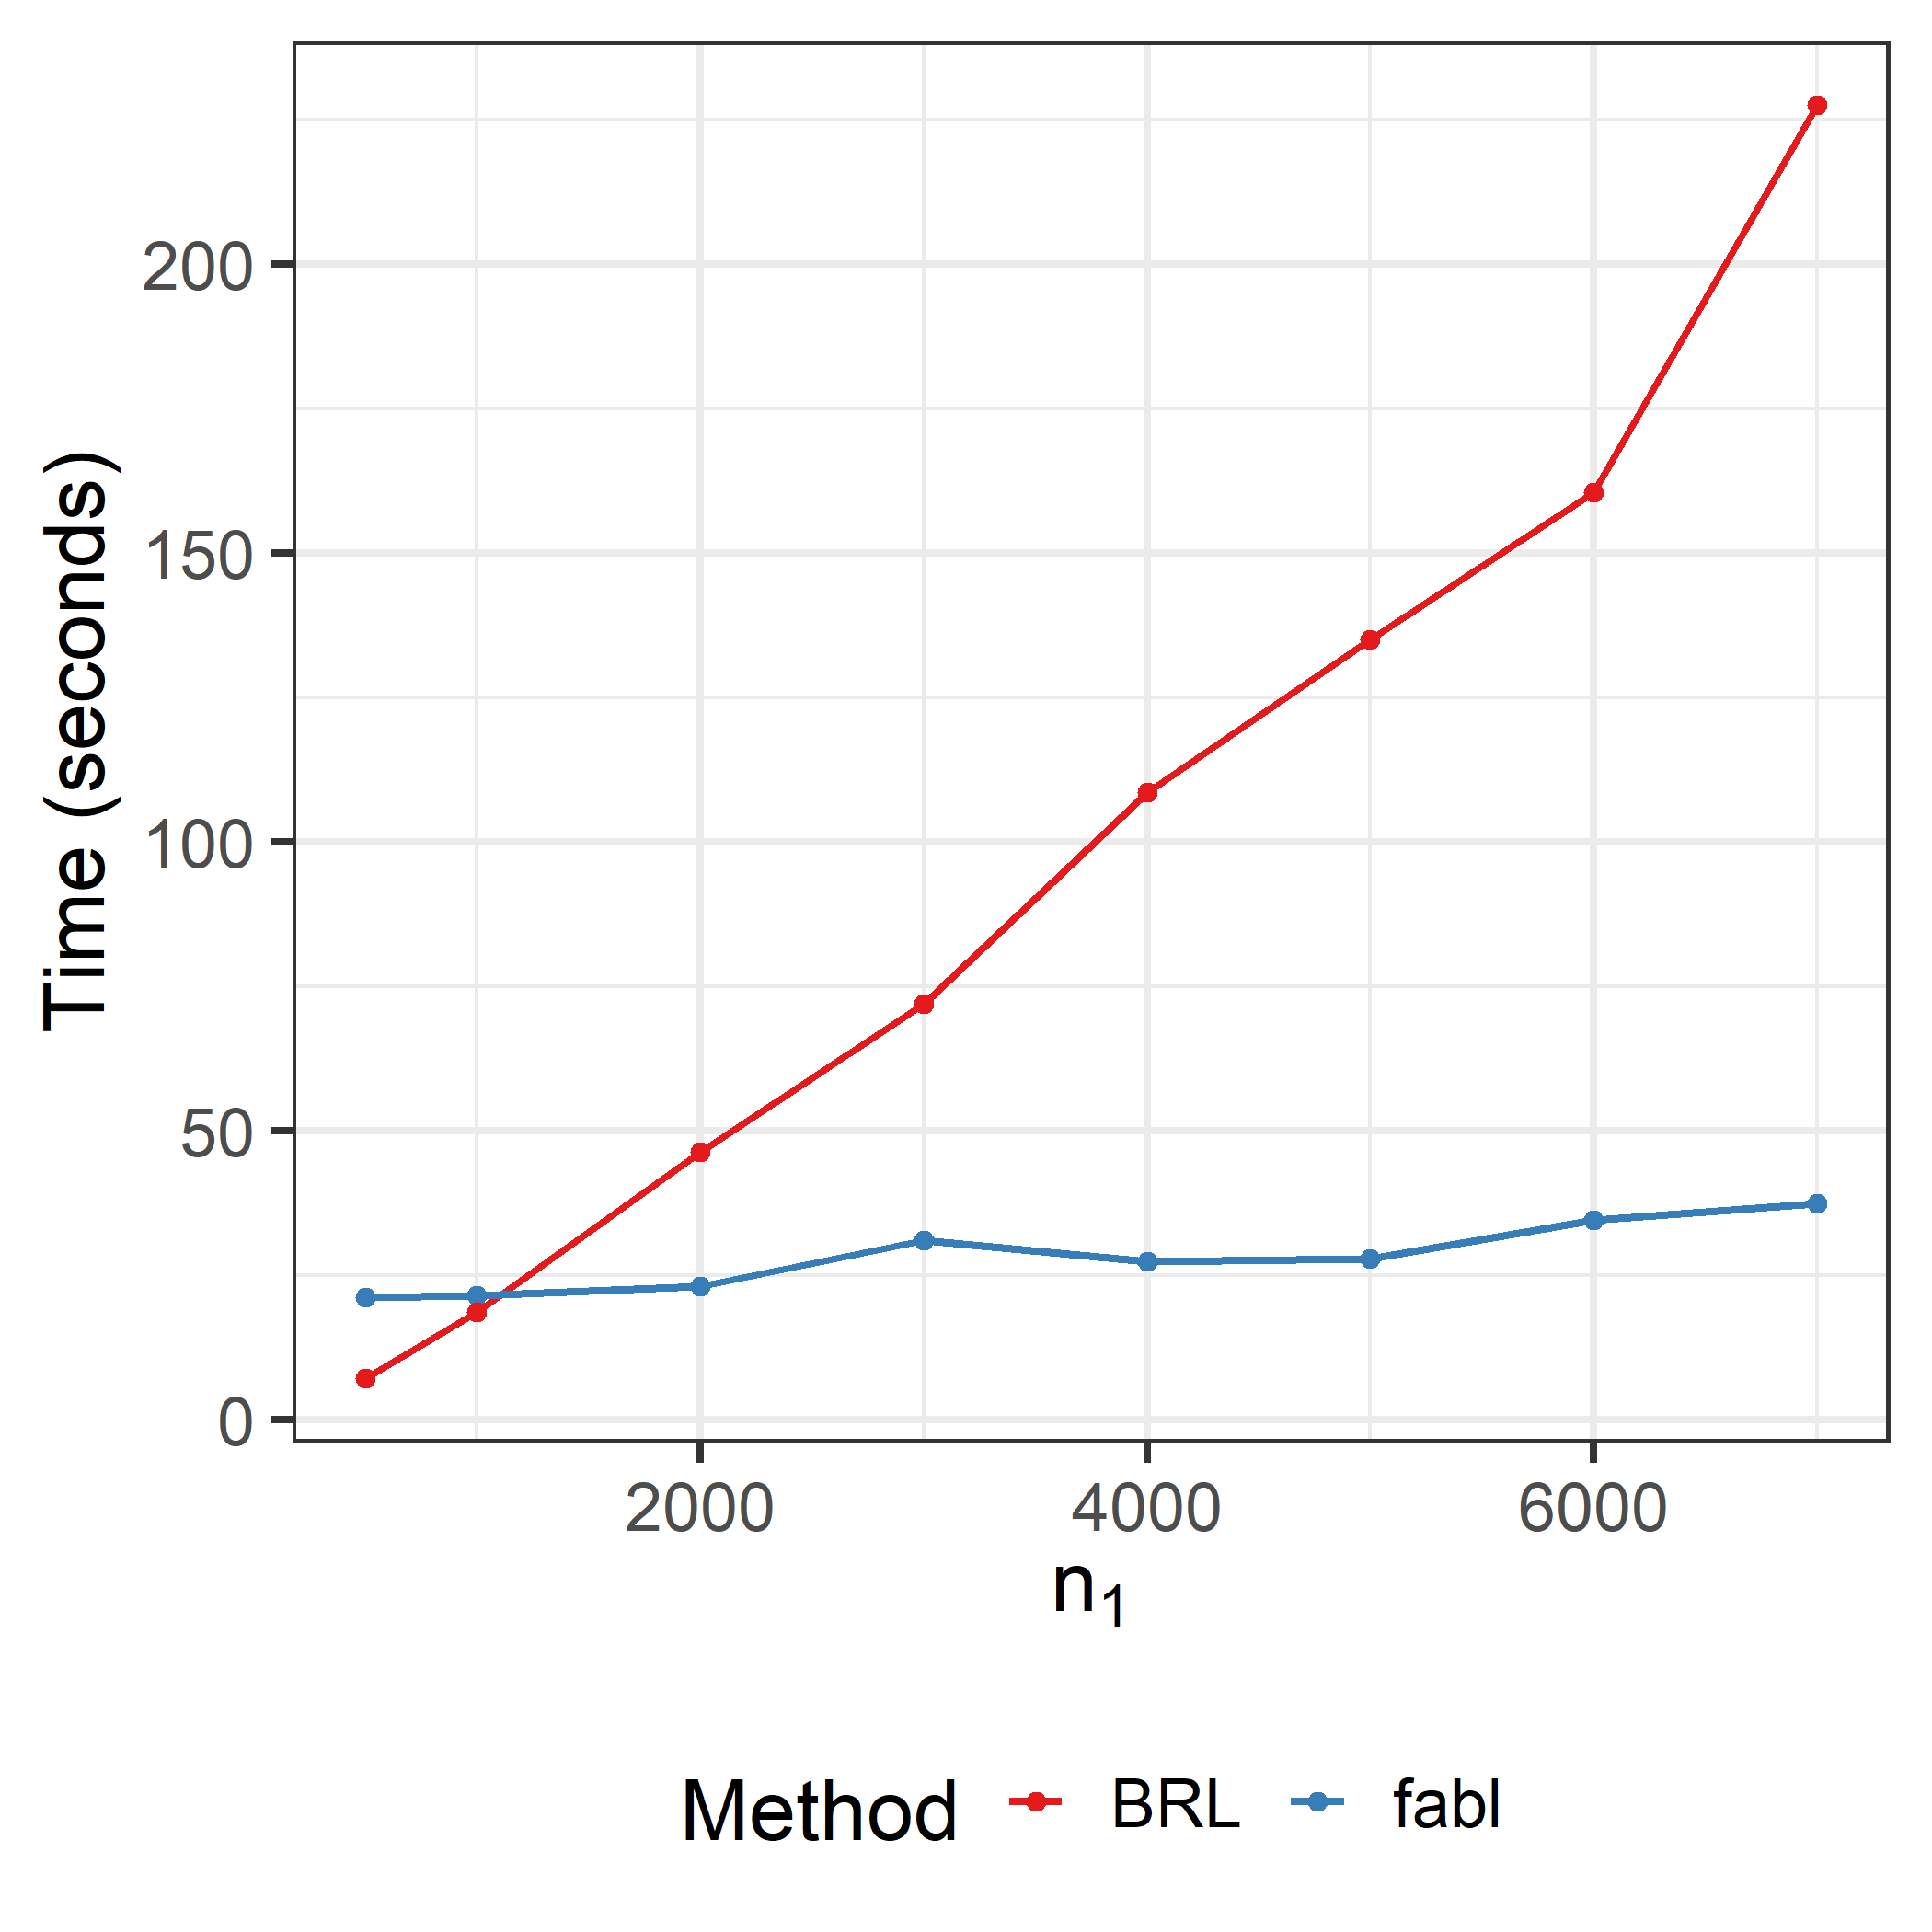
\includegraphics[width=0.6\textwidth]{finalFigures/figures/speed_plot_fixed_nB_slides2} 
%		 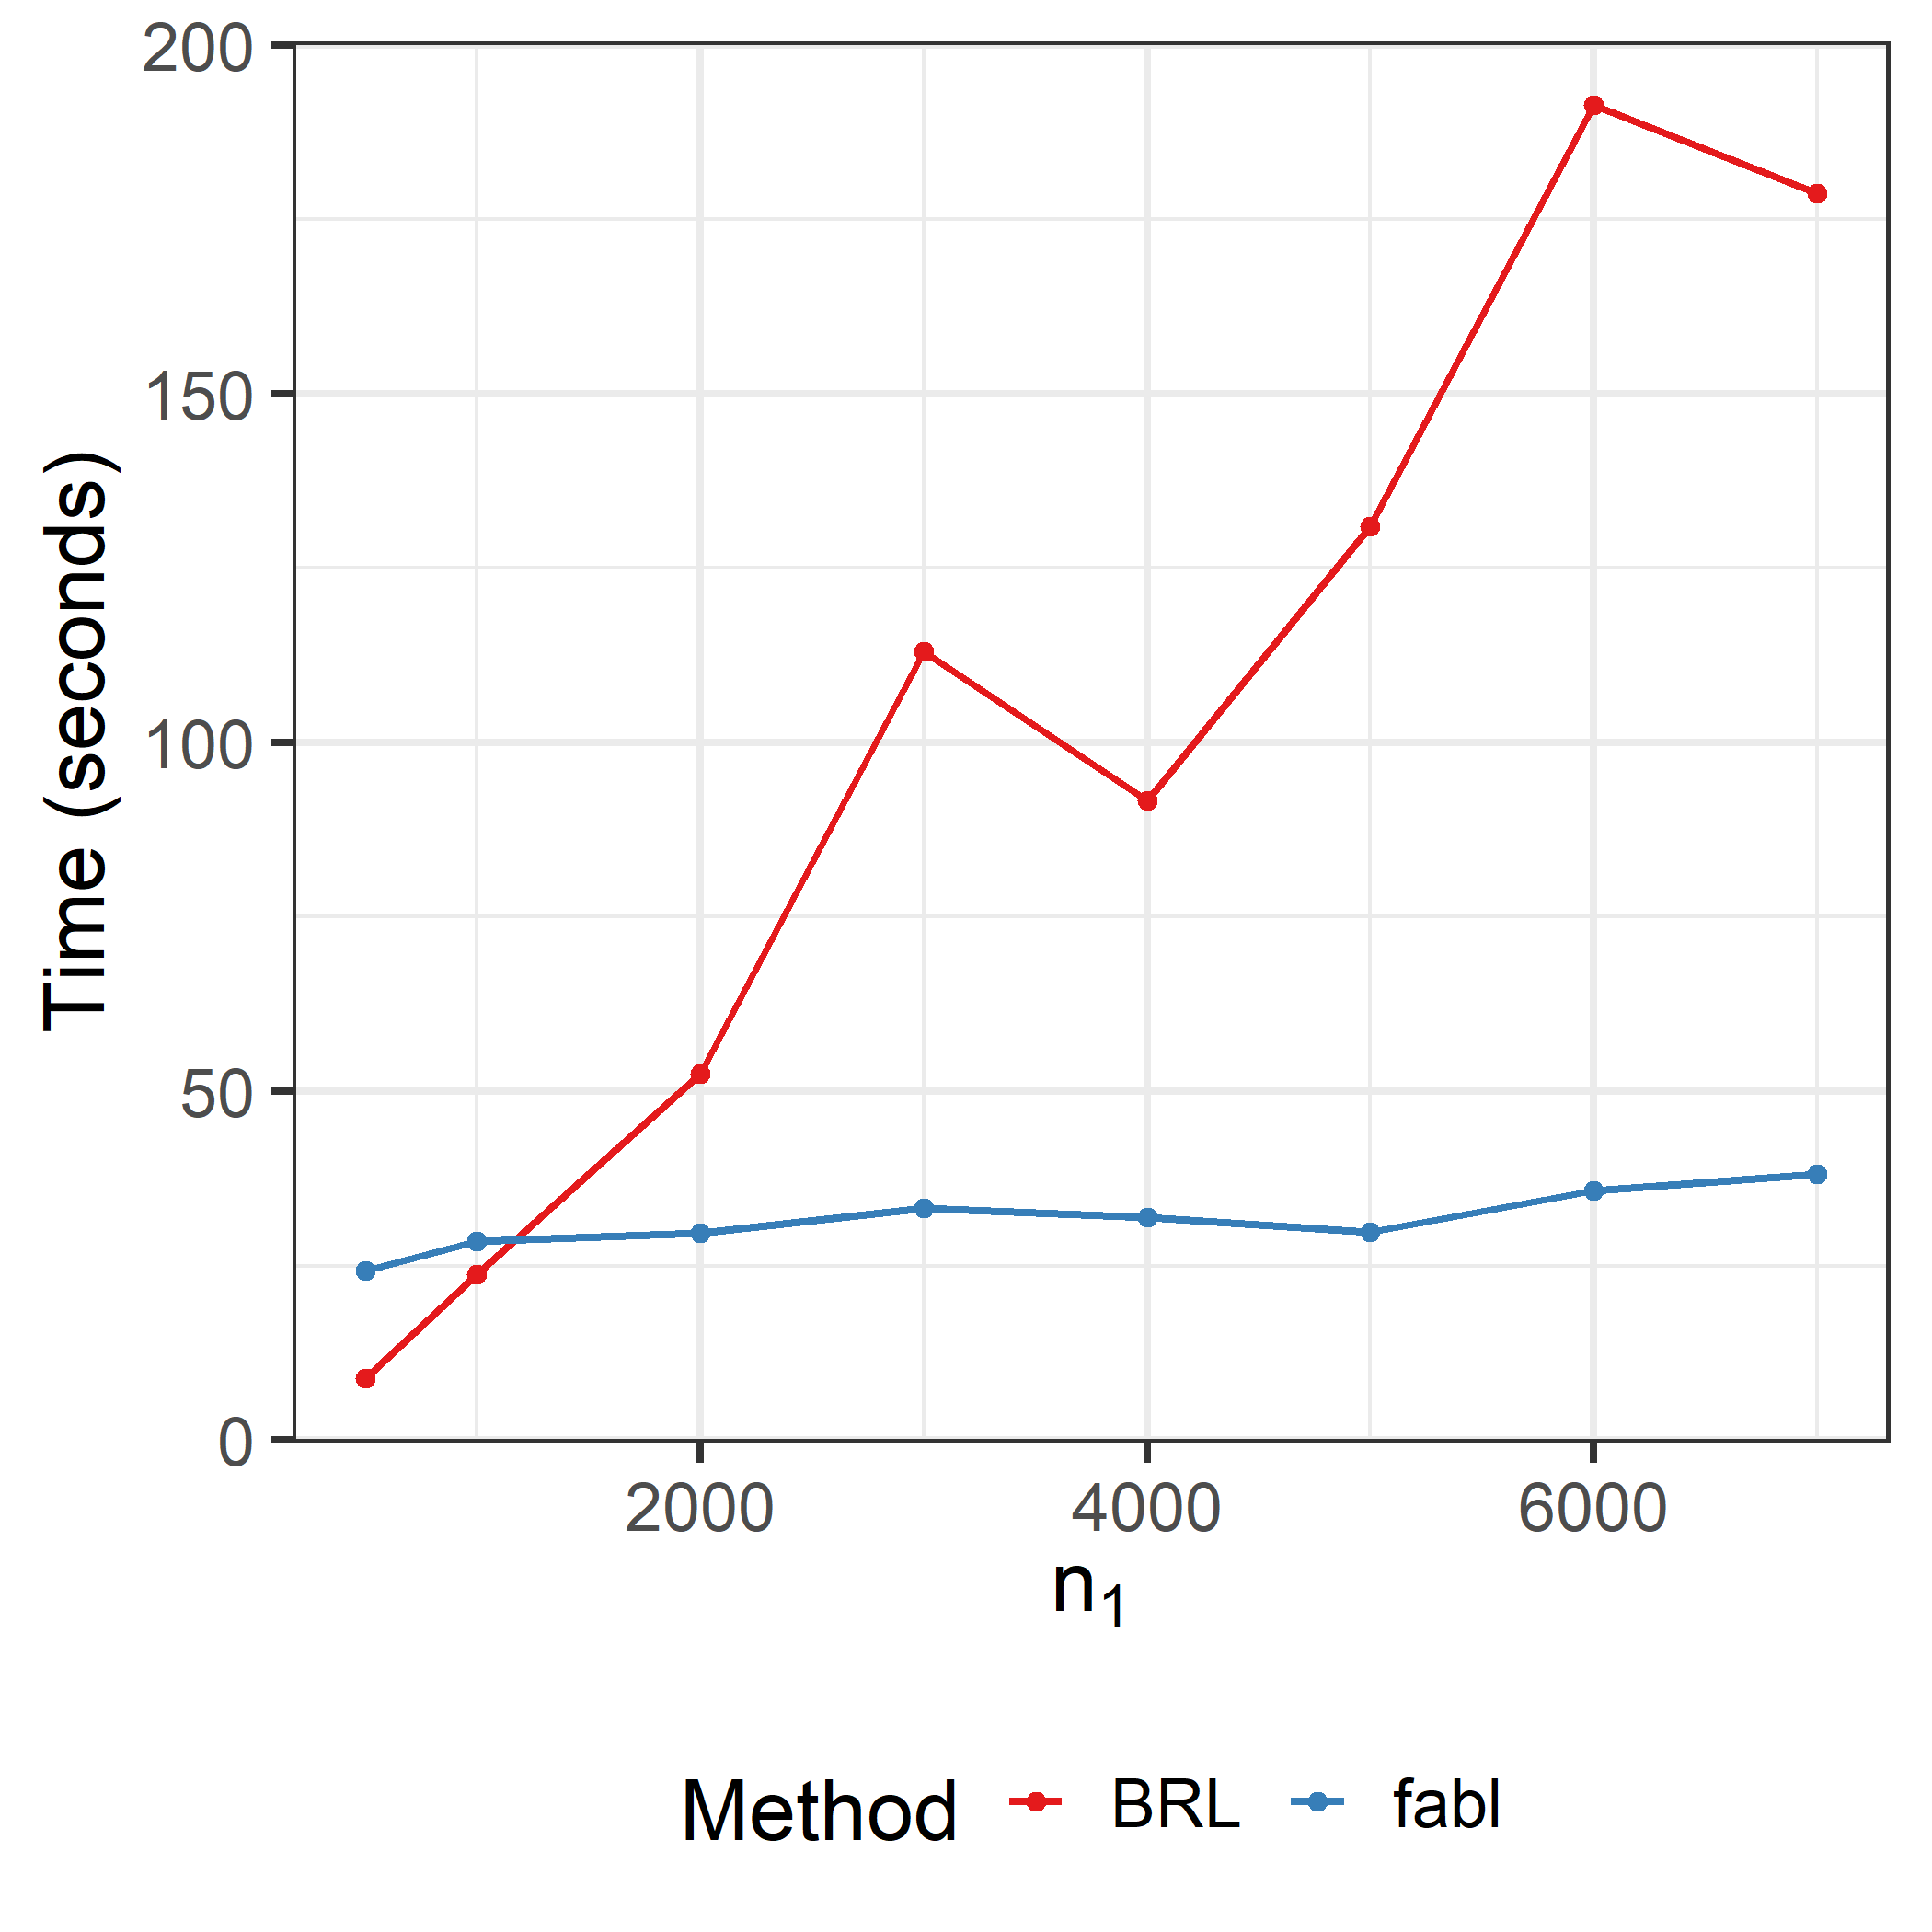
\includegraphics[width=0.6\textwidth]{../notes/figures/speed_plot_fixed_nB_slides2} 
%			\caption{Run-time for \texttt{BRL} and \texttt{fabl} to run 1000 Gibbs iterations in simulation study in Appendix \ref{app:appendix-speed}, including hashing step for \texttt{fabl}, with increasing $n_A$ and $n_B$ fixed at 500. We see linear growth in run-time for \texttt{BRL}, and near constant run-time for \texttt{fabl}.}\label{fig:app-speed2}
%		\end{center}
%	\end{figure}
%
%\clearpage
%	
%	\hypertarget{appendix-es}{%
%		\section{Traceplots for El Salvador Case Study}\label{app:appendix-es}}
%	
%	\begin{figure}[!h]
%		\begin{center}
%%		         \includegraphics[width=0.6\textwidth]{finalFigures/el_salvador/overlap_trace} 
%		\includegraphics[width=0.6\textwidth]{../notes/figures/el_salvador/overlap_trace} 
%			\caption{Traceplot for number of matches found across data files in El Salvador case study.} \label{fig:overlap_trace}
%		\end{center}
%	\end{figure}
%	
%	\begin{figure}[!h]
%		\begin{center}
%%		         \includegraphics[width=0.6\textwidth]{finalFigures/el_salvador/m_trace} 
%			\includegraphics[width=0.6\textwidth]{../notes/figures/el_salvador/m_trace} 
%			\caption{Traceplot for $\bm{m}$ parameter in El Salvador case study.} 
%			\label{fig:m_trace}
%		\end{center}
%	\end{figure}
%	
%	\begin{figure}[!h]
%		\begin{center}
%%		        \includegraphics[width=0.6\textwidth]{finalFigures/el_salvador/u_trace} 
%		\includegraphics[width=0.6\textwidth]{../notes/figures/el_salvador/u_trace} 
%			\caption{Traceplot for $\bm{u}$ parameter in El Salvador case study.} 
%			\label{fig:u_trace}
%		\end{center}
%	\end{figure}
\end{document}
